\pdfoutput=1

\documentclass{article}

\usepackage[preprint]{tmlr}

\def\month{07}
\def\year{2026}

\usepackage{amsmath,amssymb,amsthm}
\usepackage{booktabs}
\usepackage{graphicx}
\usepackage{hyperref}
\usepackage{xcolor}
\usepackage{array}
\usepackage{enumitem}
\usepackage{multirow}
\usepackage{cleveref}
\usepackage{float}
\graphicspath{{figures/}}

\newcommand{\Gr}{\mathrm{Gr}}
\newcommand{\IIA}{\mathrm{IIA}}
\newcommand{\R}{\mathbb{R}}
\newcommand{\Z}{\mathbb{Z}}
\newcommand{\dgr}{d_{\Gr}}
\newcommand{\Span}{\mathrm{span}}
\newcommand{\KL}{D_\mathrm{KL}}
\newcommand{\JS}{D_\mathrm{JS}}
\DeclareMathOperator{\diag}{diag}

\newtheorem{assumption}{Assumption}
\newtheorem{proposition}{Proposition}

\title{When Does Linear Causal Abstraction Work?\\
Mapping the Boundary on the Grassmannian}

\author{
\name Elliot Tower \\
\email elliot@elliottower.ai
}

\begin{document}
\maketitle

\begin{abstract}
Distributed Alignment Search (DAS) identifies low-dimensional linear subspaces
that mediate model behavior under interchange interventions, implicitly assuming
that the relevant causal variable lives on the Grassmannian manifold
$\Gr(k,d)$. When does this assumption hold, and what happens when it fails?

We construct an atlas of 14 modular arithmetic operations across four prime
moduli ($p = 53, 97, 113, 211$) and multiple model depths (1, 2, and 4
layers). We report four findings.
\textbf{(1)}~Whether a model develops Grassmannian causal variables is
governed by grokking, but grokking itself depends on the interaction between
operation, prime, and depth: grokking rates range from 8\% ($p{=}53$) to
71\% ($p{=}211$), and depth has a non-monotonic effect. Two robust extremes
emerge---operations that never grok regardless of conditions (squaring,
cubing) and operations that always grok given sufficient data
(addition, multiplication)---with remaining operations on a difficulty
spectrum whose boundaries shift with dataset size and model capacity.
\textbf{(2)}~Linear DAS returns $\IIA = 0.0$ on fully grokked modular
addition, while memorized models achieve $\IIA \geq 0.86$ without geometric
structure, demonstrating that IIA alone cannot distinguish genuine causal
variables from lookup tables.
\textbf{(3)}~A Structured pi-SAE---a label-conditional sparse autoencoder
with end-to-end intervention training---recovers nonlinear causal variables
where DAS fails, achieving strict IIA~$\geq 0.90$ on five of six GPT-2
language tasks at $k{=}1$ (vs.\ DAS's $0.00$--$0.52$), and
IIA~$= 0.993$ on held-out sentence templates with diversity ratio $0.53$
(cross-distribution generalization). Unconstrained
nonlinear baselines achieve perfect IIA vacuously via degenerate
encoder-decoders, confirming the non-linear representation dilemma; we
introduce \emph{intervention faithfulness} metrics (diversity ratio,
distributional fidelity) that expose this failure mode and provide a
constructive resolution via generative constraints.
\textbf{(4)}~Mechanistic analysis reveals that nonlinearity is necessary for
grokking but attention is not (DMF + ReLU groks 18$\times$ faster); that
Fourier structure emerges \emph{after} generalization, not before it; that
weight-space SVD predicts causal geometry without optimization
($\IIA = 0.999$ vs.\ DAS's $0.150$); and that the causal subspace identity
is degenerate---10 seeds produce orthogonal subspaces that all support
equally valid interventions.
\end{abstract}

\section{Introduction}
\label{sec:intro}

Mechanistic interpretability seeks to identify causally active,
human-understandable variables inside neural networks. Causal abstraction
formalizes this goal: a model variable is ``causal'' if interventions on its
internal representation behave like interventions on a high-level algorithmic
variable \citep{geiger2021causal}. Distributed Alignment Search (DAS)
operationalizes causal abstraction by learning a rotation $Q \in \R^{d \times k}$
that identifies a $k$-dimensional subspace of the residual stream. Swapping the
in-subspace component between two inputs and measuring whether the model
produces the corresponding counterfactual output yields Interchange Intervention
Accuracy (IIA) \citep{geiger2023finding}.

DAS has been applied to syntax \citep{geiger2023finding}, arithmetic
\citep{wu2024interpretability}, and board games \citep{li2023emergent}, but
every application embeds a structural assumption: the causal variable is a
\emph{linear} subspace---a point on the Grassmannian manifold $\Gr(k,d)$. When
the true causal variable is linear, DAS recovers it. When it is not, DAS may
still return a high-IIA subspace that reflects memorization or distributional
artifacts rather than genuine causal structure.

The linearity assumption has a converse problem: relaxing it naively makes
causal abstraction vacuous. \citet{sutter2025nonlinear} prove that
unconstrained nonlinear alignment maps can align any network to any algorithm
at $\IIA = 1.0$, even random models. The question is therefore not simply
whether DAS ``works'' in the narrow sense of achieving high IIA---it almost
always does. We ask: \textbf{when does the linear assumption hold?} Is the
subspace DAS recovers a genuine Grassmannian point with the geometric
properties expected of a linear causal variable, or an artifact of searching
in the wrong function class? And when it fails, \textbf{can a structured
nonlinear method recover the causal variable without falling into the
vacuity trap?}

To answer these questions, we construct an atlas of 14 operations over $\Z_p$
spanning the boundary between linear and nonlinear causal structure. We train
transformers across four prime moduli ($p = 53, 97, 113, 211$) and three
depths (1, 2, 4 layers), fit DAS at multiple subspace dimensions, and
evaluate the recovered subspace with three diagnostics beyond IIA:
equivariance under the operation's symmetry group, circle geometry of the DAS
projection, and intrinsic dimension from $k$-sweeps. When DAS fails, we apply
a Structured pi-SAE \citep{narayanaswamy2017learning}---a label-conditional
sparse autoencoder---showing that nonlinear causal variables exist even where
linear methods return zero.

The atlas reveals that Grassmannian causal structure is governed by grokking,
but grokking itself is not a fixed property of the operation: it depends on
dataset size and model depth. At $p{=}53$, only 1 of 13 operations groks; at
$p{=}211$, 10 of 14 do. Depth has a non-monotonic effect: 2-layer models
unlock grokking for operations like subtraction and absolute difference that
fail at 1 layer, but 4-layer models regress on these same operations while
the robust grokkers persist. Two robust
extremes persist across all conditions: squaring and cubing never grok, while
addition and multiplication always grok at $p \geq 97$. Between these
extremes, operations sit on a difficulty spectrum whose position shifts with
prime and depth.

Grokked modular addition returns $\IIA = 0.0$ under linear DAS despite having
learned the correct algorithm, while memorized models achieve
$\IIA \geq 0.86$ without geometric structure---demonstrating that IIA alone
cannot distinguish genuine causal variables from lookup tables.
A 10-seed stability experiment confirms that stochastic grokking is
reproducible: composite addition groks at 5 of 10 seeds at $p{=}113$,
while power groks at 0 of 10. A Structured pi-SAE with end-to-end
intervention training recovers nonlinear causal variables where DAS fails.
To confirm this method generalizes beyond grokking, we validate on six
GPT-2 language tasks, achieving strict IIA~$\geq 0.90$ on five of six at
$k{=}1$ (Table~\ref{tab:nlp_results}), and IIA~$= 0.993$ on held-out
sentence templates (Table~\ref{tab:cross_dist}).

Beyond the atlas, we ask \textbf{how does grokking create causal structure?}
Architecture ablations show that nonlinearity is necessary but attention is
not. Fine-grained trajectory analysis reveals that Fourier structure emerges
\emph{after} generalization, and that weight-space SVD predicts causal
geometry without optimization. The causal subspace itself is gauge
freedom---the model does not prefer a canonical subspace.

\paragraph{Contributions.}
\begin{enumerate}[leftmargin=*]
\item \textbf{Multi-condition atlas.} We construct an atlas of 14 operations
  across 4 prime moduli and multiple model depths,
  mapping the boundary of linear causal abstraction. The boundary is not a
  fixed property of the operation: grokking rates range from 8\% ($p{=}53$)
  to 71\% ($p{=}211$), depth has a non-monotonic effect (2-layer helps,
  4-layer regresses for boundary operations), and only the
  extremes (squaring/cubing vs.\ addition/multiplication) are robust across
  all conditions. Stochastic grokking---seed-dependent outcomes for
  operations near the boundary---provides the cleanest evidence that
  generalization, not architecture, governs causal geometry.
\item \textbf{IIA insufficiency and faithfulness metrics.} We show that
  high IIA is compatible with memorization ($\IIA = 1.0$ at $k{=}4$ for
  non-grokking operations) and with degenerate encoder-decoders (NL-DAS
  achieves $\IIA = 1.0$ via lookup tables). We introduce equivariance
  testing, intervention diversity ratio, and continuous distributional
  measures (KL, JS) as necessary complements, organized into a four-level
  evaluation hierarchy.
\item \textbf{Structured pi-SAE.} A label-conditional sparse autoencoder
  with end-to-end intervention training recovers nonlinear causal
  variables where DAS fails entirely. The generative structure prevents
  the degenerate solutions that plague unconstrained nonlinear baselines.
  Validated on six GPT-2 language tasks (strict IIA $\geq 0.90$ on five
  of six at $k{=}1$) and on cross-distribution splits (IIA $= 0.993$ on
  held-out templates, honest IIA $\approx 0$ on disjoint entity sets).
\item \textbf{Mechanistic analysis.} Nonlinearity is necessary for grokking
  but attention is not (DMF + ReLU groks 18$\times$ faster). Fourier
  structure lags generalization by $\sim$1{,}000 epochs. Weight-space SVD
  achieves $\IIA = 0.999$ without optimization. The causal subspace identity
  is degenerate (10 seeds, pairwise overlap $\approx 0.008$).
\end{enumerate}


\section{Background}
\label{sec:background}

\subsection{Causal abstraction and DAS}

Let $h(x) \in \R^d$ be an intermediate activation for input $x$. DAS searches
for an orthonormal $Q \in \R^{d \times k}$ whose column span defines a causal
subspace. Given a base input $x_b$ and source input $x_s$, the interchange
intervention replaces the in-subspace component:
\begin{equation}
h' = h_b - QQ^\top h_b + QQ^\top h_s .
\label{eq:intervention}
\end{equation}
IIA measures the fraction of interventions for which the model's output matches
the target counterfactual. High IIA indicates causal sufficiency: the subspace
contains enough information to drive behavior under interchange. But sufficiency
is not validity. A subspace may score high IIA because it encodes a memorized
lookup table, because correlated directions redundantly encode the same label, or
because the intervention distribution is too easy.
\citet{makelov2024illusion} demonstrated this concretely: subspace activation
patching can produce interpretability illusions where dormant pathways inflate IIA
without reflecting genuine causal structure. Our central claim is that IIA must be
paired with geometric diagnostics that test whether the subspace is a genuine
linear causal variable rather than an artifact of the linear function class.

\subsection{The Grassmannian manifold}
\label{sec:grassmannian_background}

The Grassmannian $\Gr(k,d)$ is the set of all $k$-dimensional linear subspaces
of $\R^d$. A DAS solution $Q \in \R^{d \times k}$ represents a point
$[Q] = \Span(Q)$ on this manifold; any $QR$ for $R \in O(k)$ represents the
same point. The geodesic distance between two subspaces is determined by their
\emph{principal angles}: if $Q_1, Q_2$ have orthonormal columns, the singular
values of $Q_1^\top Q_2$ are $\cos \theta_i$, and the geodesic distance is
\begin{equation}
\dgr([Q_1],[Q_2]) = \left(\sum_i \theta_i^2\right)^{1/2}
\label{eq:geodesic}
\end{equation}
\citep{edelman1998geometry, absil2008optimization}. Every application of DAS is
implicitly a search on this manifold. The question ``does DAS work?'' is
really ``does the true causal variable live on $\Gr(k,d)$?'' When it does, DAS
recovers a meaningful point. When it does not, DAS still returns a point on
$\Gr(k,d)$, but that point may be an artifact.

\subsection{Structured disentangled generative models}
\label{sec:structured_vae}

Semi-supervised deep generative models \citep{narayanaswamy2017learning} extend
the VAE framework \citep{kingma2014auto} by partitioning the latent space into
supervised and unsupervised factors. The generative model factors as
$p(x, y, z) = p(x \mid y, z) \, p(y) \, p(z)$, where $y$ is a labeled
(interpretable) variable and $z$ captures unlabeled nuisance variance. The
recognition model $q(y, z \mid x) = q(z \mid x, y) \, q(y \mid x)$ uses neural
network encoders, allowing nonlinear latent structure.

This framework is a natural generalization of DAS: DAS constrains the causal
variable to live on $\Gr(k,d)$ (a linear subspace), while the structured VAE
allows it to occupy a nonlinear manifold in activation space. The key advantage
is disentanglement: the supervised factor $y$ is trained to predict the
operation's output, while the unsupervised factor $z$ absorbs everything else.
If the causal variable is linear, the VAE encoder should learn a rotation
equivalent to DAS. If the causal variable is nonlinear (e.g., circular
structure from Fourier representations), the VAE can recover it where DAS
cannot.

The loss function combines the evidence lower bound (ELBO) with a supervised
classification term:
\begin{equation}
\mathcal{L} = \underbrace{-\mathbb{E}_{q}[\log p(x \mid y, z)]}_{\text{reconstruction}}
+ \beta \underbrace{D_\mathrm{KL}(q(y,z \mid x) \,\|\, p(y) p(z))}_{\text{regularization}}
+ \alpha \underbrace{\mathcal{L}_\text{CE}(y, \hat{y})}_{\text{supervision}}.
\label{eq:vae_loss}
\end{equation}

The encoder weights projecting to $y$ provide a linearized approximation of the
causal subspace; if this linearization has high overlap with the DAS subspace,
it confirms that the causal variable is approximately Grassmannian.

\subsection{Identifiability of the causal latent factor}
\label{sec:identifiability}

A central concern for any latent-variable method is \emph{identifiability}:
does the encoder recover the \emph{true} latent factors, or an arbitrary
reparameterization? The Structured pi-SAE architecture is designed to
approximate the conditions of iVAE \citep{khemakhem2020variational}:
(i)~the task label $y$ is an observed auxiliary variable;
(ii)~the label-conditional prior
$p(z_\text{causal} \mid y) = \mathcal{N}(\mu_y, \sigma_y^2 I)$ is an
exponential family with per-label means; (iii)~the ELBO reconstruction
loss encourages an approximately injective decoder.

\paragraph{Connection to iVAE identifiability.}
\label{prop:recovery}
If the iVAE conditions of \citet{khemakhem2020variational} hold exactly---injective
decoder, sufficient variability of per-label parameters, and exponential family
conditionals---then Theorem~1 of \citet{khemakhem2020variational} guarantees
recovery of the true latent factors up to a component-wise bijection. In
practice, neural network activations are deterministic functions of the input,
not samples from a generative model, so these conditions hold only
approximately. The ELBO encourages but does not guarantee decoder injectivity,
and the rank condition on per-label means is plausible for $p = 113$ classes
but may not hold for small datasets (e.g., the 182-class capitals task).
We therefore treat iVAE identifiability as a \emph{design motivation} rather
than a formal guarantee, and rely on empirical controls
(\S\ref{sec:nldas_vacuous}) to validate that the encoder recovers
meaningful structure.

\paragraph{Three consequences of the generative structure.}
\textbf{(1) NL-DAS violates the reconstruction constraint}:
its decoder is not reconstruction-constrained, so multiple latent codes may
map to the same activation and identifiability does not hold
(\S\ref{sec:nldas_vacuous}).
\textbf{(2) The component-wise ambiguity is harmless for IIA}:
interchange swaps $z_\text{causal}$ wholesale, so any bijection $\phi$ cancels.
\textbf{(3) Linear DAS is the special case $\phi \in O(k)$.}
When the true causal variable is linear, the structured encoder degenerates
to a rotation, matching the DAS solution.

\subsection{Grokking as a phase transition}

Grokking is a training regime in which models memorize the training set long
before generalizing \citep{power2022grokking}. Modular arithmetic models trained
with weight decay exhibit grokking reliably for some operations but not others
\citep{nanda2023progress, zhong2024clock}. \citet{gromov2023grokking} derives
an analytic solution for modular addition showing that grokked models learn
cosine weights implementing discrete Fourier transforms.
\citet{khanh2026scaling} provide a quantitative scaling law for the grokking
delay, validated over 293 runs, linking the memorization-to-generalization gap
to the ratio of weight norms before and after the transition.
Our perspective is complementary: we ask how the causal subspace recovered by
DAS changes across this transition, and whether it is deterministic or
stochastic across random seeds.
\citet{liu2023grokking} frame grokking as compression---moving from a memorized
high-complexity solution to a generalizing low-complexity one; our Grassmannian
perspective gives this compression a geometric interpretation as convergence to a
specific point on $\Gr(k,d)$.


\section{Methods}
\label{sec:methods}

\subsection{Operations and models}

We study 14 binary operations over $\Z_p$ (Table~\ref{tab:operations}), chosen
to span group actions, polynomials, piecewise functions, and non-algebraic maps.
We train transformers with $d_\text{model} = 128$, four attention heads
($d_\text{head} = 32$), and $d_\text{MLP} = 512$ on examples of the form
$(a, b, {=}) \mapsto y$. The core sweep varies three axes: prime modulus
$p \in \{53, 97, 113, 211\}$, model depth $n_\text{layers} \in \{1, 2, 4\}$,
and operation (14 types). Training uses
the standard grokking setup: 30\% train split, AdamW with learning rate
$10^{-3}$, weight decay 1.0, full-batch, and 25{,}000--80{,}000 epochs
depending on the operation (1.5$\times$ for deeper models). We classify a
model as \emph{grokked} if its final test cross-entropy is below 0.1.

\begin{table}[t]
\centering
\small
\begin{tabular}{llll}
\toprule
Operation & Formula & Category & Seeds tested \\
\midrule
Multiplication & $ab \bmod 113$ & Group action & 42, 2024 \\
Comp.\ addition & $(a{+}b) \bmod 91$ & Group action & orig, 42 \\
Subtraction & $(a{-}b) \bmod 113$ & Group action & 42 \\
Division & $a/b \bmod 113$ & Group action & 42 \\
Bitwise XOR & $a \oplus b \bmod 113$ & Group action & 42, 137, 2024 \\
\midrule
Sum of squares & $(a^2{+}b^2) \bmod 113$ & Polynomial & 42 \\
Cubic sum & $(a^3{+}b^3) \bmod 113$ & Polynomial & 42 \\
Cubing & $a^3 \bmod 113$ & Polynomial & 42 \\
Squaring & $a^2 \bmod 113$ & Polynomial & 42 \\
Polynomial & $(a^2{+}b) \bmod 113$ & Polynomial & 42 \\
Affine & $(2a{+}3b{+}5) \bmod 113$ & Polynomial & 42 \\
\midrule
Max & $\max(a,b) \bmod 113$ & Piecewise & 42 \\
Abs.\ difference & $|a{-}b| \bmod 113$ & Piecewise & 42 \\
Power & $a^b \bmod 113$ & Non-algebraic & 42, 137 \\
\bottomrule
\end{tabular}
\caption{Operation atlas. Group actions provide clean equivariance targets.
Polynomials test whether nonlinear maps admit linear causal variables. Piecewise
and non-algebraic operations probe the boundary.}
\label{tab:operations}
\end{table}

\subsection{DAS fitting and $k$-sweeps}

For each trained model, we cache residual-stream activations and train a DAS
rotation $Q \in \R^{d \times k}$ using interchange interventions for 200
gradient steps (Adam, lr $= 10^{-3}$, batch size 16 interchange pairs).
We sweep $k \in \{2, 4, 6, 8, 10, 12, 16, 20, 24, 32\}$ to
estimate the intrinsic dimension $k^*$, defined as the smallest $k$ achieving
$\IIA \geq 0.95$. Each $k$ value is an independent DAS optimization, not a
nested subspace---$k$-sweep profiles reveal whether the causal variable is
inherently low-dimensional or requires many dimensions.

\subsection{Hard-example selection for IIA}
\label{sec:hard_examples}

Standard IIA evaluation includes many ``easy'' examples where the intervention
does not change the model's top-1 prediction, inflating IIA regardless of whether
the subspace is causally valid. We define a \emph{hard example} as a
(base, source) pair where: (1) the base and source have different correct outputs
$y_b \neq y_s$, (2) the model's prediction matches the correct output for both
base and source separately, and (3) the interchange intervention at the DAS
subspace \emph{can} flip the model's prediction from $y_b$ to $y_s$. Hard IIA
measures the fraction of hard examples where the flip actually occurs. This
selection follows the methodology of constrained PCA-initialized DAS,
which showed that standard IIA saturates too easily while hard IIA reveals
genuine causal structure.

\subsection{Equivariance testing}

For operations with a natural group action, we test whether the DAS subspace
respects the algebraic symmetry. Given input $(a, b)$ with DAS projection
$z = Q^\top h(a,b)$, we construct a shifted input $(a{+}1 \bmod p, b)$ and
check whether the DAS projection rotates by $2\pi/p$ radians. The equivariant
fraction is the proportion of test inputs satisfying this rotation property.
Random orthogonal subspaces of the same dimension serve as controls; across all
operations, random-subspace equivariance is below 1\%.

\subsection{Structured VAE for nonlinear causal variables}
\label{sec:vae_method}

For each trained grokking model, we cache residual-stream activations at the
post-MLP hook and train a structured VAE with:
\begin{itemize}[leftmargin=*]
\item $z_\text{causal}$: $k$-dimensional latent factor ($k \in \{2,4,8\}$),
  semi-supervised with the operation's output label via a classification head.
\item $z_\text{nuisance}$: $m$-dimensional unsupervised factor ($m = 15$) to
  absorb non-causal variance.
\item Encoder: 2-layer MLP ($d_\text{model} \to 128 \to z$) with ReLU.
\item Decoder: 2-layer MLP ($z \to 128 \to d_\text{model}$) with ReLU.
\end{itemize}

Training uses the combined ELBO + classification loss (Eq.~\ref{eq:vae_loss})
for 300 epochs with $\beta = 1.0$, $\alpha = 10.0$, $L_1$ coefficient
$\lambda = 1.0$, and Adam optimizer with learning rate $10^{-3}$.

\paragraph{VAE-based IIA.}
We evaluate the VAE's causal subspace by performing interchange interventions in
the \emph{latent} space: given base activation $h_b$ and source activation
$h_s$, we encode both, swap $z_\text{causal}$ while keeping $z_\text{nuisance}$
from the base, decode back to activation space, and measure whether the model
produces the source's output. This is the nonlinear analogue of
Eq.~\ref{eq:intervention}: instead of $QQ^\top$ projection, we use the
encode-swap-decode path.

\paragraph{VAE equivariance.}
We test whether the VAE's $z_\text{causal}$ exhibits equivariance under additive
shifts, using the same protocol as for DAS (shift input $a \to a+1$, check
whether $z_\text{causal}$ rotates consistently). Because the VAE encoder is
nonlinear, it can represent circular structure directly in a 2D latent space.

\subsection{Nonlinear DAS baseline}
\label{sec:nldas}

To isolate the contribution of the VAE's generative structure from the benefit
of nonlinearity alone, we compare against an unconstrained nonlinear featurizer.
Given MLP encoder $f: \R^d \to \R^d$ and decoder $g: \R^d \to \R^d$, the
nonlinear DAS (NL-DAS) intervention is:
\begin{equation}
h' = g\bigl(f(h_b) - QQ^\top f(h_b) + QQ^\top f(h_s)\bigr)
\label{eq:nldas}
\end{equation}
where $Q \in \R^{d \times k}$ is learned jointly with $f$ and $g$ by maximizing
interchange accuracy. Both $f$ and $g$ use the same architecture as the VAE
encoder (2-layer MLP, 256 hidden units, ReLU), matching the VAE's representational
capacity. Crucially, NL-DAS has \emph{no reconstruction constraint}: $f$ and $g$
are trained exclusively on interchange loss and need not be (approximately)
inverse to each other.

We also evaluate NL-DAS+recon, which adds a reconstruction penalty
$\lambda \| g(f(h)) - h \|^2$ to the training loss, forcing $f$ and $g$ to
approximate mutual inverses. This tests whether the unconstrained NL-DAS result
degrades when the encoder-decoder cannot be degenerate.

\subsection{Intervention faithfulness metrics}
\label{sec:faithfulness_metrics}

Binary IIA measures \emph{interchange effectiveness}: does swapping the
subspace component change the model's output to match the source? But
effectiveness alone does not imply that the intervention is \emph{faithful}---that
it modifies only the targeted causal variable while preserving all other
information. A method that achieves IIA~=~1.0 by overwriting the entire
activation with a class-specific template is effective but not faithful.

We introduce four complementary metrics to evaluate intervention faithfulness:

\paragraph{Continuous distributional metrics.}
Binary IIA saturates at 1.0 whenever the top-1 prediction flips, hiding
differences in intervention quality. We measure the full distributional impact:
\begin{itemize}[leftmargin=*]
\item \textbf{KL divergence}: $\KL(p_\text{clean} \| p_\text{iv})$, where
  $p_\text{clean}$ and $p_\text{iv}$ are the softmax distributions before and
  after intervention. Lower KL means the intervention preserves more of the
  clean distribution beyond the swapped variable.
\item \textbf{Jensen-Shannon divergence}: the symmetric alternative
  $\JS = \frac{1}{2}\KL(p \| m) + \frac{1}{2}\KL(q \| m)$ where $m = (p+q)/2$.
  Bounded in $[0, \ln 2]$, more stable than KL when distributions have disjoint
  support.
\item \textbf{Probability difference}: $p_\text{iv}(y_s) - p_\text{iv}(y_b)$,
  a continuous analog of binary IIA that captures the model's confidence margin,
  not just top-1 agreement.
\item \textbf{Normalized logit difference}:
  $\frac{l_\text{iv}(y_s) - l_\text{iv}(y_b)}{|l_\text{clean}(y_s) - l_\text{clean}(y_b)|}$,
  where $l$ denotes logits. A value of 1.0 means the intervention reproduces the
  clean model's margin exactly; values $\gg 1$ or $\ll 0$ indicate distortion.
\end{itemize}

\paragraph{Intervention diversity.}
For each source label $y_s$, we compute the standard deviation of the intervened
activations $h'$ across all base inputs with the same source. If the decoder
produces the same $h'$ regardless of which base input was used---varying only
with $y_s$---the intervention is a lookup table: it does not preserve
base-specific nuisance information. We define the \emph{diversity ratio}:
\begin{equation}
\rho = \frac{\mathbb{E}_{y_s}\bigl[\text{std}(h'_{y_s})\bigr]}
            {\mathbb{E}_{y_s}\bigl[\text{std}(h_{y_s})\bigr]}
\label{eq:diversity_ratio}
\end{equation}
where the numerator is over intervened activations sharing source label $y_s$
and the denominator is over the corresponding natural source activations.
$\rho \approx 0$ indicates a lookup table (all intervened activations for the
same $y_s$ collapse to a single point). $\rho \approx 1$ indicates the
intervention preserves the natural variation within each class.

\paragraph{Reconstruction fidelity.}
For encoder-decoder methods (NL-DAS, VAE), we measure $\|g(f(h)) - h\|^2$ on
held-out activations. A high reconstruction MSE with high IIA is a warning sign:
the decoder may be ``hallucinating'' the correct output rather than faithfully
reconstructing the activation with a modified causal component.
The generative constraint is not merely a regularizer---it is a necessary
condition for identifiability (Proposition~\ref{prop:recovery}), as shown
empirically by pi-VAE's failure despite having the correct prior direction
(Table~\ref{tab:ablation}).

\subsection{Cross-distribution generalization}
\label{sec:cross_distribution}

Standard train/test splits draw from the same distribution. For IOI on GPT-2, we
additionally evaluate under distribution shift: (1)~\textbf{disjoint names}---train
on one set of proper names, evaluate on a completely disjoint set; and
(2)~\textbf{disjoint templates}---train on sentence templates 1--3, evaluate on
templates 4--5 plus novel hard templates. A method that generalizes under
distribution shift is finding a genuine causal variable; one that fails is
exploiting distributional regularities in the training set.


\section{Results}
\label{sec:results}

\subsection{The atlas: a grokking-governed spectrum}

At a single prime ($p{=}113$, 1-layer), the 14 operations appeared to partition
into three classes (Table~\ref{tab:main_results}).
\citet{furuta2024modular} study multiple operations at fixed prime and depth,
finding asymmetries in subtraction and Fourier bias in multiplication; our
multi-modulus sweep extends this to show that the partition itself is not fixed:
grokking depends on the interaction between operation, prime, and depth
(Table~\ref{tab:multimod}).

\begin{table}[t]
\centering
\small
\setlength{\tabcolsep}{3pt}
\begin{tabular}{lcccccl}
\toprule
Operation & Grok & Loss & IIA($k{=}2$) & $k^*$ & Equiv. & Class \\
\midrule
\multicolumn{7}{l}{\textit{Always Grassmannian (at $p{=}113$)}} \\
Multiplication & \checkmark & 0.000 & 1.000 & 2 & 0.995 & Always \\
Subtraction & \checkmark & 0.000 & 1.000 & 2 & 1.000 & Always \\
Division & \checkmark & 0.000 & 1.000 & 2 & 1.000 & Always \\
Bitwise XOR & \checkmark & 0.003 & 1.000 & 2 & 1.000 & Always \\
Cubic sum & \checkmark & 0.000 & 1.000 & 2 & 1.000 & Always \\
Sum of squares & \checkmark & 0.005 & 1.000 & 2 & 0.987 & Always \\
Max & \checkmark & 0.074 & 0.960 & 2 & 0.957 & Always \\
\midrule
\multicolumn{7}{l}{\textit{Stochastic}} \\
Comp.\ addition$^*$ & \checkmark & 0.000 & --- & --- & 0.998 & Stochastic \\
Comp.\ addition (s42) & $\times$ & 10.207 & 0.800 & 6 & 0.110 & Stochastic \\
Power (s137) & \checkmark & 0.088 & 0.940 & 4 & 0.965 & Stochastic \\
Power (s42) & $\times$ & 1.143 & 0.980 & 2 & 0.665 & Stochastic \\
\midrule
\multicolumn{7}{l}{\textit{Never Grassmannian (at $p{=}113$)}} \\
Cubing & $\times$ & 9.765 & 0.857 & 4 & 0.509 & Never \\
Squaring & $\times$ & 7.808 & 0.857 & 4 & 0.314 & Never \\
Abs.\ difference & $\times$ & 1.835 & 0.800 & $>$32 & 0.189 & Never \\
Polynomial & $\times$ & 21.550 & 0.720 & $>$32 & 0.015 & Never \\
Affine & $\times$ & 26.209 & 0.780 & $>$32 & 0.026 & Never \\
\bottomrule
\end{tabular}
\caption{Atlas results at $p{=}113$ (1-layer). $k^*$ is the
smallest $k$ achieving $\IIA \geq 0.95$.
$^*$Original seed (unknown value); k-sweep not recorded.
Table~\ref{tab:multimod} shows how this partition shifts across primes.}
\label{tab:main_results}
\end{table}

\begin{table}[t]
\centering
\small
\setlength{\tabcolsep}{4pt}
\begin{tabular}{l cccc cc}
\toprule
Operation & $p{=}53$ & $p{=}97$ & $p{=}113$ & $p{=}211$ & 2L & 4L \\
\midrule
\multicolumn{7}{l}{\textit{Robust grokkers}} \\
Addition         & ---  & \checkmark & \checkmark & \checkmark & \checkmark & \checkmark \\
Multiplication   & ---  & \checkmark & \checkmark & \checkmark & \checkmark & \checkmark \\
Bitwise XOR      & \checkmark & \checkmark & \checkmark & \checkmark & \checkmark & \checkmark \\
Sum of squares   & $\sim$  & \checkmark & \checkmark & \checkmark & \checkmark & \checkmark \\
\midrule
\multicolumn{7}{l}{\textit{Difficulty spectrum (condition-dependent)}} \\
Division         & ---  & \checkmark & ---  & \checkmark & \checkmark & --- \\
Subtraction      & ---  & ---  & ---  & \checkmark & \checkmark & --- \\
Max              & $\sim$ & $\sim$ & \checkmark & \checkmark & $\sim$ & --- \\
Min              & $\sim$ & $\sim$ & \checkmark & \checkmark & $\sim$ & $\sim$ \\
Abs.\ difference & ---  & ---  & ---  & \checkmark & \checkmark & --- \\
Comp.\ addition  & --- & \checkmark & --- & ---  & \checkmark$^*$ & --- \\
Power            & ---  & ---  & ---  & \checkmark & --- & --- \\
Affine           & ---  & ---  & ---  & ---  & --- & --- \\
\midrule
\multicolumn{7}{l}{\textit{Robust non-grokkers}} \\
Squaring         & ---  & ---  & ---  & ---  & --- & --- \\
Cubing           & ---  & ---  & ---  & ---  & --- & --- \\
\midrule
\multicolumn{7}{l}{\textit{Aggregate grokking rate}} \\
& 1/13 & 6/14 & 6/14 & 10/14 & & \\
& (8\%) & (43\%) & (43\%) & (71\%) & & \\
\bottomrule
\end{tabular}
\caption{Grokking across primes and depth. 1-layer results across four
primes; 2L and 4L columns at $p{=}113$.
\checkmark = grokked (test CE $< 0.1$); $\sim$ = near-grokked
(acc $> 0.97$ but CE $> 0.1$); --- = did not grok.
$^*$Comp.\ addition groks at $p{=}97$ (1L and 2L) but not $p{=}113$ or
$p{=}211$ at seed 42---consistent with stochastic classification.
Note that 4-layer models do \emph{not} uniformly improve over 2-layer:
subtraction, abs.\ difference, and division grok at 2L but regress at 4L.}
\label{tab:multimod}
\end{table}

Three patterns emerge from the multi-condition sweep. First, grokking rate
scales with dataset size: at $p{=}53$ ($\sim$800 training pairs), only
bitwise XOR groks; at $p{=}211$ ($\sim$13{,}000 pairs), 10 of 14 operations
do. This suggests that many operations classified as ``never Grassmannian''
at $p{=}113$ simply had insufficient data to cross the grokking threshold.

Second, the relationship between depth and grokking is non-monotonic. At
$p{=}113$ with 2 layers, subtraction, absolute difference, and division all
grok, whereas none of these grok with 1 layer at the same prime. But at 4
layers, these same operations \emph{regress}---none grok despite the
additional capacity. Only the robust grokkers (addition, multiplication,
bitwise XOR, sum of squares) maintain grokking at 4 layers. The 2-layer
sweet spot suggests that moderate depth helps by providing compositional
capacity, while excessive depth hinders generalization by enabling more
complex memorization strategies. This non-monotonic pattern is consistent
with the observation that deeper networks have higher effective capacity for
memorization \citep{arpit2017closer}, which competes with the generalization
pathway that grokking requires.

Third, two robust extremes persist across all conditions. Squaring and
cubing never grok at any prime or depth tested---their output structure
(quadratic/cubic residues) appears fundamentally resistant to the
generalization transition. Conversely, addition and multiplication grok at
every prime $\geq 97$ and at every depth, consistent with their clean
group-homomorphic algebraic structure.

\begin{figure}[t]
\centering
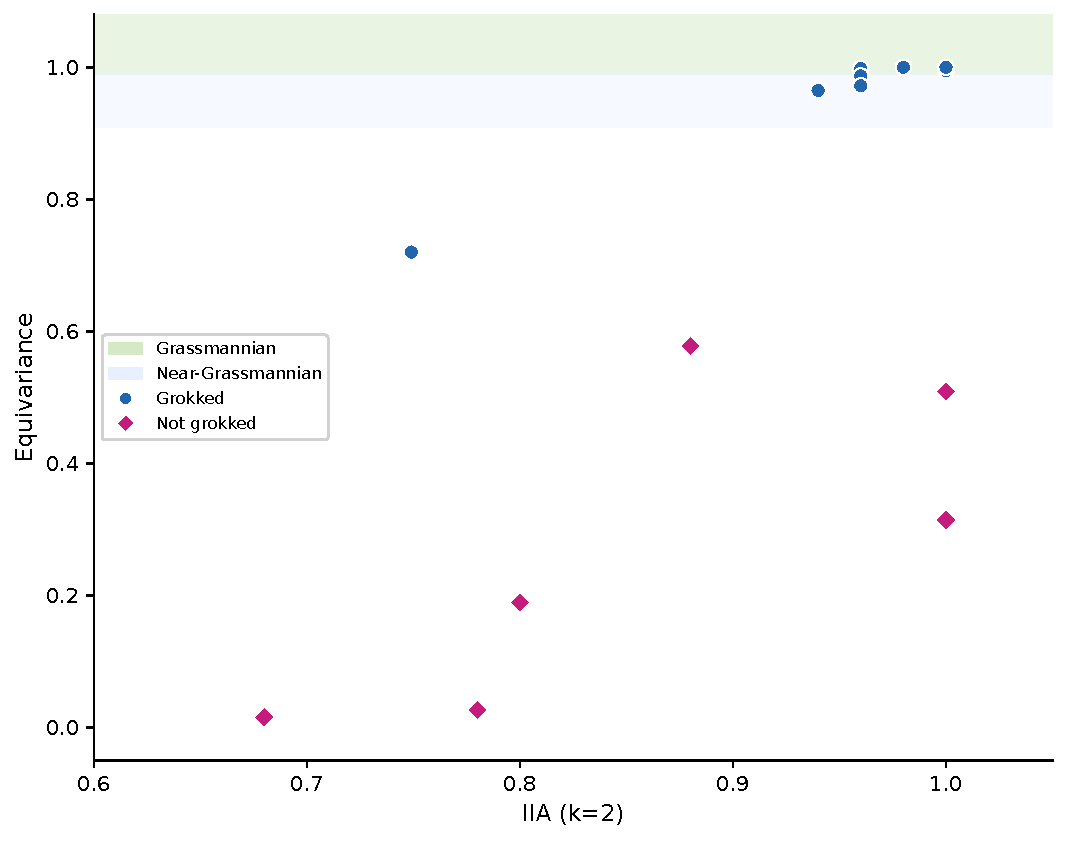
\includegraphics[width=\linewidth]{fig2c_iia_vs_equiv_grokked}
\caption{IIA ($k{=}2$) vs.\ equivariance across all operations at $p{=}113$.
Grokked operations (blue circles) cluster in the Grassmannian and
Near-Grassmannian bands; non-grokked operations (pink diamonds) scatter
below. High IIA alone does not guarantee geometric structure---several
non-grokked operations achieve IIA $> 0.8$ with equivariance $< 0.5$.}
\label{fig:iia_vs_equiv}
\end{figure}

\subsection{Linear DAS fails on grokked modular addition}
\label{sec:linear_das_fails}

The starkest evidence that the Grassmannian assumption can fail even for correct,
generalizing models comes from modular addition. We train DAS at
$k \in \{2, 4, 8, 16\}$ on residual-stream activations from a fully grokked
model (test loss $< 10^{-7}$, test accuracy 100\%). At \emph{every} subspace
dimension, DAS returns $\IIA = 0.0$---not low, but exactly zero.

This is not a failure of DAS optimization. The model has learned the correct
modular addition algorithm via Fourier representations \citep{nanda2023progress}:
the ``identity'' of each number $a$ is encoded as
$(\cos 2\pi f a / p, \sin 2\pi f a / p)$ for key frequencies $f$. This
representation lives on $S^1$ (a circle embedded in $\R^d$), not on a linear
subspace of $\R^d$. DAS searches $\Gr(k,d)$ for a flat plane that captures a
curved manifold---a category error, not an optimization failure.

This motivates the Structured pi-SAE approach (\S\ref{sec:vae_results}):
a nonlinear sparse encoder can map the circular representation to a structured
latent space where interchange interventions succeed. On grokked addition, the
Structured pi-SAE achieves IIA~=~1.0 at $k{=}2$, confirming that the causal
variable exists but is nonlinear.

\begin{figure}[t]
\centering
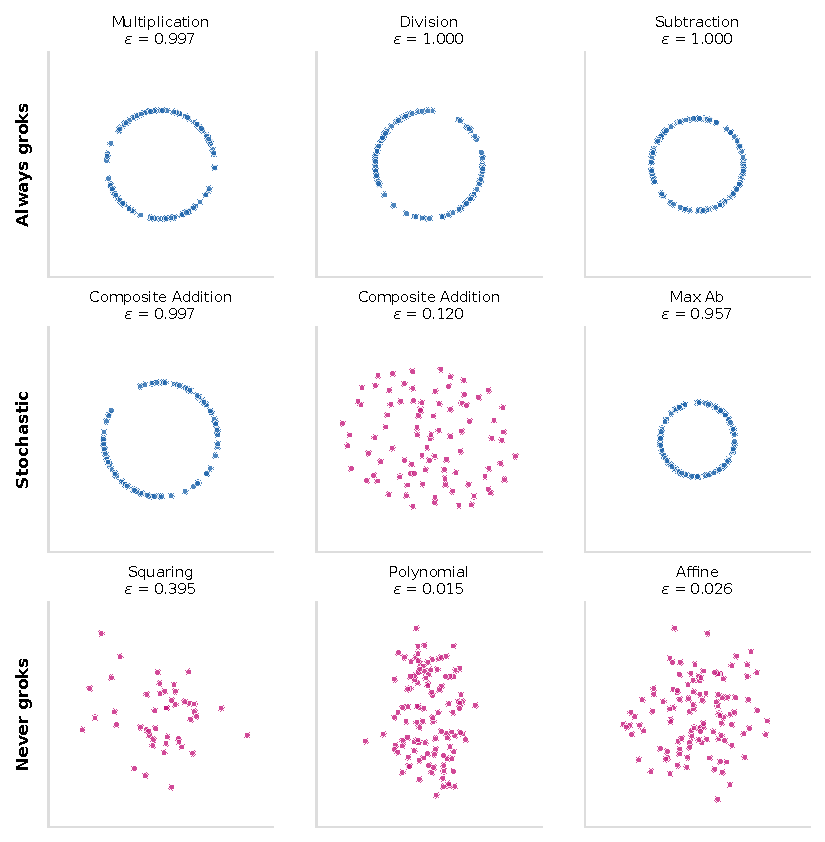
\includegraphics[width=\linewidth]{fig20v2_real_circles_compact}
\caption{DAS 2D projections of label centroids across three grokking
classes. Grokked operations (top two rows, blue) produce centroids
arranged on a circle in the learned subspace, reflecting the group
action's rotational structure. Non-grokked operations (bottom row, pink)
produce unstructured scatter. The stochastic row shows composite
addition under two seeds: one grokked (circular), one not (scattered).}
\label{fig:circle_geometry}
\end{figure}

\subsection{Stochastic grokking: the same operation, opposite outcomes}
\label{sec:stochastic}

The multi-modulus sweep reveals that stochastic grokking is not an anomaly
confined to two operations---it is a pervasive feature of the boundary region.
A 10-seed stability experiment at $p{=}113$ confirms this directly: composite
addition ($a + b \bmod 91$) groks at exactly 5 of 10 seeds, while power
($a^b \bmod 113$) groks at 0 of 10. The same operation exhibits different
grokking behavior across primes---composite addition groks at $p{=}97$ but
not at $p{=}211$ (at seed 42)---confirming that the boundary is genuinely
stochastic rather than a deterministic function of the operation's algebraic
structure.

The multi-modulus data also reveals that operations previously classified as
``never Grassmannian'' were misclassified. Bitwise XOR groks at all four
primes tested, including $p{=}53$ where almost nothing else groks. Sum of
squares groks at three of four primes. These operations were classified as
``never'' based on a single prime ($p{=}113$) where they happened not to
grok---a classification error that the multi-condition sweep corrects.
The lesson is methodological: single-condition classifications of grokking
behavior are unreliable for operations near the boundary.

\begin{figure}[t]
\centering
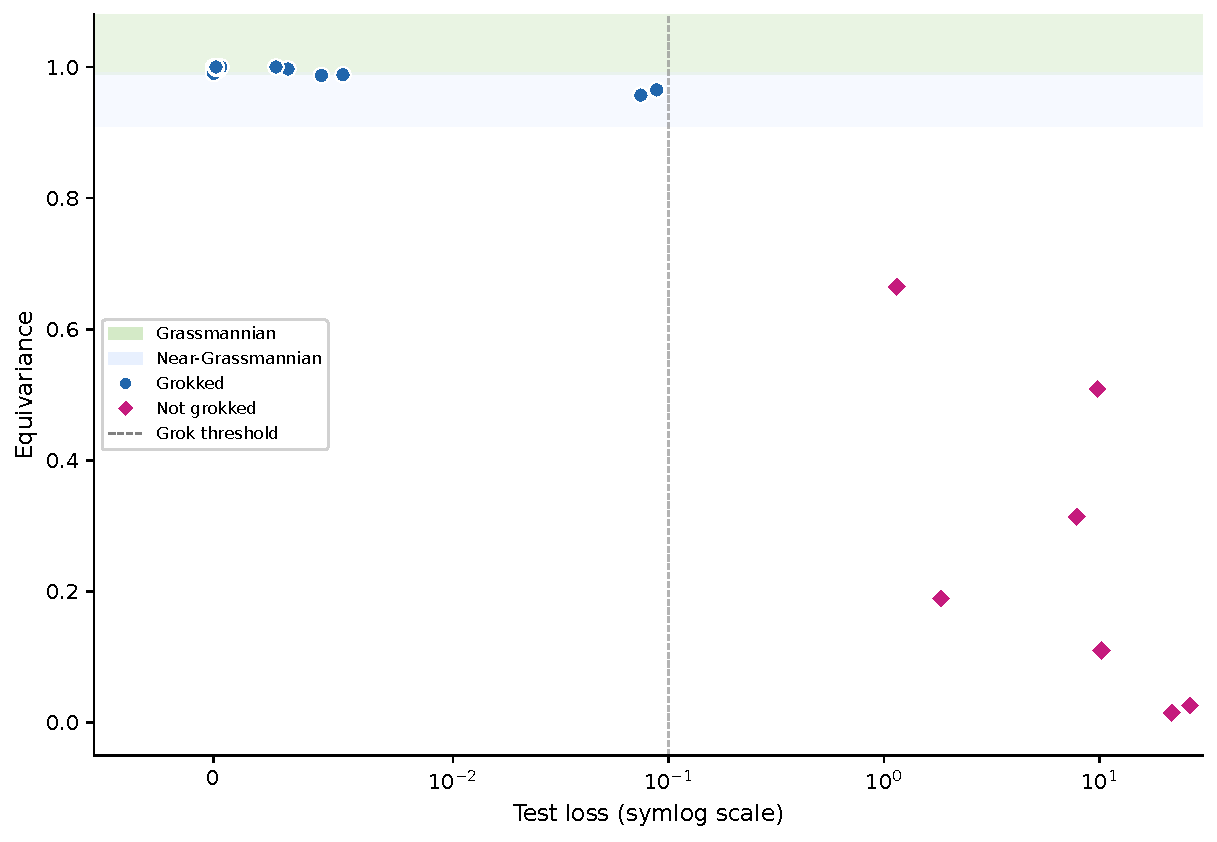
\includegraphics[width=\linewidth]{fig8c_loss_vs_equiv_grokked}
\caption{Test loss vs.\ equivariance across all operation--seed pairs.
The dashed line marks the grokking threshold (test loss $= 0.1$).
Grokked operations (blue, left of threshold) cluster at high
equivariance; non-grokked operations (pink, right) scatter across the
full range. Equivariance values shown use the angular tolerance metric
(\S\ref{sec:limitations}); intervention-based re-measurement
(Appendix~\ref{app:equiv_test}) confirms the qualitative separation.}
\label{fig:loss_vs_equiv}
\end{figure}

\subsection{Memorization artifacts: high IIA, no structure}
\label{sec:memorization}

Squaring and cubing achieve $\IIA = 0.86$ at $k = 2$ and $\IIA = 1.0$ by $k = 4$
without grokking (test losses 7.8 and 9.8). Equivariance exposes the artifact:
31.4\% for squaring and 50.9\% for cubing, far below the $>$95\% threshold. The
lesson: \textbf{high IIA with low-$k$ saturation is compatible with a lookup
table}. ``Works for interchange'' and ``is a Grassmannian causal variable'' are
different claims.

\subsection{$k$-sweep profiles correlate with equivariance}

Grassmannian variables saturate at $\IIA \approx 1.0$ by $k = 4$: their causal
structure is inherently 2-dimensional. Non-Grassmannian variables show gradual IIA
growth that may not reach 1.0 even at $k = 32$. Polynomial reaches
$\IIA = 0.72$ at $k = 2$ and requires $k \geq 8$ to approach 0.90.

\begin{figure}[t]
\centering
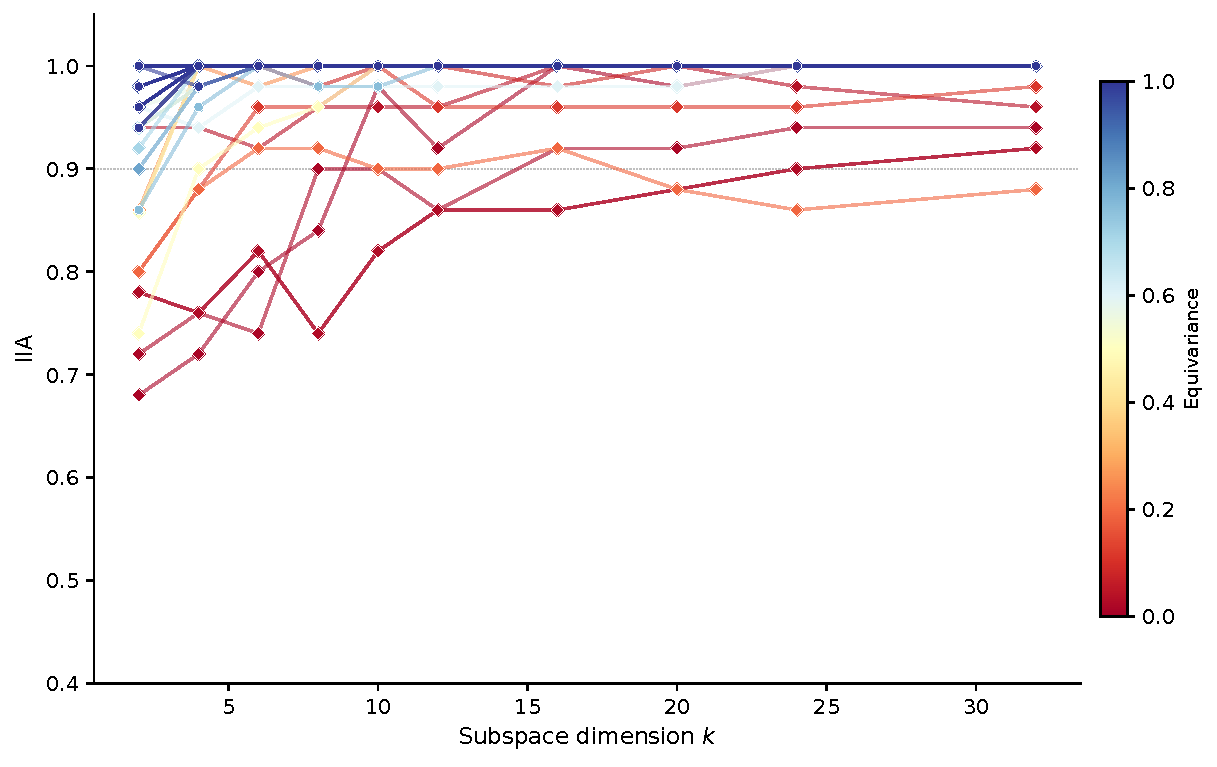
\includegraphics[width=\linewidth]{fig23b_k_sweep_equiv_colored}
\caption{IIA as a function of subspace dimension $k$ for all operations,
colored by equivariance. High-equivariance operations (dark blue)
saturate at $\IIA \approx 1.0$ by $k = 2$--$4$; low-equivariance
operations (red) show gradual growth that plateaus well below 1.0.
The separation between the two regimes is visible at every $k$.}
\label{fig:k_sweep}
\end{figure}

\subsection{Structured pi-SAE recovers nonlinear causal variables}
\label{sec:vae_results}

We upgrade the vanilla structured VAE to a \textbf{Structured pi-SAE}: a
label-conditional sparse autoencoder that partitions the latent space into
$z_\text{causal}$ (supervised, $L_1$-penalized) and $z_\text{nuisance}$
(unsupervised). The ``pi'' denotes the label-conditional prior from
\citet{narayanaswamy2017learning}; the ``SAE'' denotes $L_1$ sparsity on
$z_\text{causal}$ with an expansion factor of $8\times$ (so $k$ causal
dimensions expand to $8k$ sparse features). This combines the identifiability
guarantees of auxiliary supervision \citep{khemakhem2020variational} with the
interpretability benefits of sparse dictionary learning
\citep{bricken2023towards}.

\paragraph{The $2 \times 2$ ablation.}
Both components---structured prior and sparsity---are necessary
(Table~\ref{tab:ablation}). On grokking tasks: (1)~the plain SAE (no
label-conditional prior) achieves IIA~=~1.0 on addition but degrades on harder
operations (multiplication~0.72, quartic sum~0.32); (2)~the pi-VAE (structured
prior, no sparsity) achieves IIA~$\approx$~0 across all operations;
(3)~\emph{only} the Structured pi-SAE achieves IIA~=~1.0 uniformly across all
grokked operations and IIA~$\approx$~0 on all non-grokked operations.

\begin{table}[t]
\centering
\small
\setlength{\tabcolsep}{4pt}
\begin{tabular}{@{}l|cc|cc@{}}
\toprule
& \multicolumn{2}{c|}{\textbf{Plain prior} $\mathcal{N}(0,I)$}
& \multicolumn{2}{c}{\textbf{Structured prior} $p(z \mid y)$} \\
\textbf{Operation} & VAE & SAE & pi-VAE & \textbf{Str.\ pi-SAE} \\
\midrule
\multicolumn{5}{l}{\textit{Grokked}} \\
Addition       & 0.02 & 1.00 & 0.00 & \textbf{1.00} \\
Multiplication & 0.00 & 0.72 & 0.00 & \textbf{1.00} \\
Quartic sum    & 0.02 & 0.32 & 0.00 & \textbf{1.00} \\
IOI (GPT-2)    & 0.56 & 0.83 & 0.95 & \textbf{0.98} \\
\midrule
\multicolumn{5}{l}{\textit{Non-grokked (correct answer: $\approx 0$)}} \\
Mixed product  & 0.03 & 0.01 & 0.01 & 0.04 \\
Squaring       & 0.00 & 0.00 & 0.00 & 0.00 \\
\bottomrule
\end{tabular}
\caption{$2{\times}2$ ablation: IIA at $k{=}2$.
Plain SAE works on addition but degrades on harder operations (multiplication
$0.72$, quartic sum $0.32$) because without the structured prior, the sparse
encoder has no target direction.  pi-VAE (structured prior, no sparsity)
achieves $0.00$ on grokked operations---the prior provides the right
direction but without sparsity the encoder spreads the causal signal across
all dimensions, which cannot be cleanly swapped.  Only Structured pi-SAE
achieves $1.00$ uniformly on all grokked operations and $\leq 0.04$ on all
non-grokked operations.}
\label{tab:ablation}
\end{table}

\paragraph{Reconstruction MSE as a falsifiability criterion.}
For non-grokked operations, reconstruction MSE is $11$--$24$; for grokked
operations, $0.6$--$1.2$.  High MSE with near-zero IIA means the model has
\emph{no structured causal variable to recover}---not that the method
failed.  This diagnostic is unavailable for NL-DAS, which returns IIA $=
0.6$--$0.8$ on non-grokked operations (false positives) because it has no
reconstruction constraint.

\paragraph{End-to-end intervention training.}
For language model tasks where the causal structure is more complex, we add an
\textbf{end-to-end (E2E) intervention CE loss}: after swapping $z_\text{causal}$
and decoding, we run the intervened activation through the remaining layers and
compute $-\log p(y_s \mid h')$. This differentiable objective directly
optimizes for intervention success, analogous to how DAS trains on interchange
accuracy. Training proceeds in two phases: 200 epochs of reconstruction +
classification warmup, followed by E2E intervention training with an additive
intervention $h' = h_b + \text{dec}(z_\text{swap}) - \text{dec}(z_\text{orig})$
that cancels reconstruction error.

\paragraph{Validation on GPT-2 language tasks.}
The Structured pi-SAE was developed to recover nonlinear causal variables in
grokking models. A natural concern is whether it overfits to the specific
geometry of modular arithmetic. To test generalization, we evaluate on six
tasks from the MIB benchmark \citep{prakash2024mib} at layer~8 of GPT-2-small,
where DAS is the established baseline (Table~\ref{tab:nlp_results}).

\begin{table}[t]
\centering
\small
\setlength{\tabcolsep}{4pt}
\begin{tabular}{lcccc}
\toprule
\textbf{Task} & \textbf{DAS} & \textbf{DAS (strict)} & \textbf{E2E} & \textbf{E2E (strict)} \\
\midrule
IOI            & 0.19 & 0.19 & \textbf{1.00} & \textbf{1.00} \\
Gender bias    & 0.62 & 0.52 & \textbf{1.00} & \textbf{1.00} \\
Greater-than   & 0.93 & 0.28 & \textbf{1.00} & \textbf{1.00} \\
SVA            & 0.92 & 0.00 & \textbf{1.00} & \textbf{1.00} \\
Hypernymy      & 0.07 & 0.02 & \textbf{0.97} & \textbf{0.90} \\
Capitals$^\dagger$ & 0.12 & ---  & \textbf{0.51} & \textbf{0.26} \\
\bottomrule
\end{tabular}
\caption{Standard and strict IIA at $k{=}1$ on six GPT-2 language tasks
(layer~8, additive intervention). Structured pi-SAE with E2E training
dominates DAS on all six tasks. $^\dagger$Capitals has 182 classes with
only 190 examples ($\approx$1 per class), limiting classifier training.}
\label{tab:nlp_results}
\end{table}

The Structured pi-SAE with E2E training matches or exceeds DAS on all six
GPT-2 tasks at $k{=}1$, confirming that the method is not specific to
grokking geometry. On five of six tasks, E2E achieves strict IIA $\geq 0.90$;
on IOI, gender bias, greater-than, and SVA it reaches 1.00. The sole
exception is capitals, where the dataset contains 182 classes with only 190
examples, limiting classifier training. On hypernymy, E2E achieves
IIA~=~0.97 at $k{=}1$---$14\times$ better than DAS (0.07)---and DAS's strict
IIA on SVA is exactly 0.00 despite standard IIA of 0.92, revealing that DAS
shifts probability mass toward the correct token without ever making it the
argmax. These results serve as a sanity check: the Structured pi-SAE is a
strict generalization of DAS (matching it where linear structure suffices,
exceeding it where nonlinear structure is needed), not a special-case method.

\paragraph{Capacity comparison.}
The methods differ substantially in parameter count
(Table~\ref{tab:params}). DAS learns only the rotation $Q$; Pi-SAE adds
an encoder-decoder with reconstruction constraints; NL-DAS adds an MLP
featurizer without constraints. Pi-SAE E2E uses the same architecture
as Pi-SAE but trains with intervention loss end-to-end. The Pi-SAE's
additional capacity is spent on reconstruction and regularization, not
on memorizing intervention pairs---as the diversity ratio confirms.

\begin{table}[t]
\centering
\small
\begin{tabular}{lrl}
\toprule
Method & Parameters & Constraints \\
\midrule
DAS         & 768     & None (linear rotation) \\
NL-DAS      & $\sim$787K  & None (end-to-end IIA only) \\
Pi-SAE      & $\sim$414K  & ELBO + KL + causal/nuisance split \\
Pi-SAE E2E  & $\sim$414K  & ELBO + KL + split + IIA \\
\bottomrule
\end{tabular}
\caption{Parameter counts at $k{=}1$ on GPT-2 ($d = 768$, hidden $= 512$,
  latent $= 16$). NL-DAS has $1.9\times$ the parameters of Pi-SAE with
  zero structural constraints, enabling the lookup-table failure mode.}
\label{tab:params}
\end{table}

On IOI \citep{wang2022interpretability}, NL-DAS achieves IIA~$= 1.00$,
but the diversity ratio $\rho \approx 0.05$ (vs.\ $\rho \approx 0.89$ for the
pi-SAE) exposes it as vacuous (Table~\ref{tab:nldas_vacuous}).

\subsection{Unconstrained nonlinear DAS is vacuous}
\label{sec:nldas_vacuous}

A natural response to DAS's linearity constraint is to prepend an MLP
featurizer: learn a nonlinear coordinate system in which the causal variable
\emph{becomes} linear, then apply standard DAS. This approach---which we call
NL-DAS (\S\ref{sec:nldas})---achieves IIA~=~1.000 on IOI at $k = 1$, compared
to DAS's 0.183. This looks like a dramatic improvement. It is not.

\paragraph{The lookup-table failure mode.}
NL-DAS is trained end-to-end on interchange loss with no reconstruction
constraint. The encoder $f$ and decoder $g$ need not be approximate inverses,
and the training objective provides no incentive for them to be. This creates a
degenerate solution: $f$ maps every activation to a space where the first
coordinate encodes the class label and the remaining coordinates are arbitrary;
$g$ ignores the base-specific content entirely and produces a ``canonical
activation for class $y_s$'' regardless of which base input was used.

The intervention diversity ratio (\S\ref{sec:faithfulness_metrics}) exposes this
failure. Table~\ref{tab:nldas_vacuous} reports results for IOI and two
grokking operations (addition, multiplication mod 113) across $k \in \{1, 2, 4\}$;
squaring did not grok within 80{,}000 epochs.

\begin{table}[t]
\centering
\small
\setlength{\tabcolsep}{3pt}
\begin{tabular}{lc rrrr rr}
\toprule
Task & $k$ & DAS & NL-DAS & NL-DAS+r & VAE & $\rho_\text{NL}$ & $\rho_\text{VAE}$ \\
\midrule
IOI & 1 & 0.183 & 1.000 & 0.867 & 1.000 & 0.05 & 0.83 \\
IOI & 2 & 0.322 & 1.000 & 0.700 & 0.989 & 0.05 & 0.89 \\
IOI & 4 & 0.572 & 1.000 & 0.811 & 0.989 & 0.05 & 0.92 \\
\midrule
Addition & 1 & 0.006 & 0.083 & 0.028 & 1.000 & 0.12 & 1.00 \\
Addition & 2 & 0.022 & 0.422 & 0.039 & 1.000 & 0.29 & 1.00 \\
Addition & 4 & 0.283 & 0.689 & 0.033 & 1.000 & 0.43 & 1.00 \\
\midrule
Mult.\ & 1 & 0.028 & 0.239 & 0.028 & 1.000 & 0.65 & 1.00 \\
Mult.\ & 2 & 0.072 & 0.544 & 0.111 & 1.000 & 1.00 & 1.00 \\
Mult.\ & 4 & 0.283 & 0.933 & 0.372 & 1.000 & 1.12 & 0.99 \\
\midrule
Squaring & $\dagger$ & \multicolumn{6}{c}{\emph{did not grok ($\text{acc} = 0.00$)}} \\
\bottomrule
\end{tabular}
\caption{NL-DAS achieves high IIA by learning degenerate encoder-decoders.
  The VAE column reports Structured pi-SAE results.
  $\rho$ is the intervention diversity ratio (Eq.~\ref{eq:diversity_ratio});
  NL-DAS+r adds a reconstruction penalty ($\lambda_\text{recon} = 0.1$).
  $\dagger$Squaring ($x^2 \bmod 113$) failed to grok within 80{,}000 epochs
  at all tested $k$.
  All controls (random labels, reconstruction-only, untrained, unconstrained
  plain VAE) achieve IIA~$< 0.09$, confirming the Structured pi-SAE is not
  cheating.}
\label{tab:nldas_vacuous}
\end{table}

Two lines of evidence support this:

\begin{enumerate}[leftmargin=*]
\item \textbf{Controls rule out the structured VAE cheating.} Random-label VAE
  (IIA $\leq 0.02$), reconstruction-only VAE with $\alpha = 0$
  (IIA $\leq 0.005$), untrained VAE (IIA = 0.000), and an unconstrained plain
  VAE with no causal/nuisance split (IIA $\leq 0.08$) all fail. The structured
  VAE's success requires correct supervision \emph{and} the
  causal-nuisance partition. NL-DAS lacks the reconstruction constraint
  that prevents degenerate solutions; without inductive biases, unsupervised
  disentanglement is impossible \citep{locatello2019challenging}.

\item \textbf{The structured prior and reconstruction constraint are
  necessary, not optional.} The ELBO forces the decoder to produce
  activations close to the original, the KL regularization prevents
  encoder collapse, and the causal-nuisance partition ensures that
  base-specific information is preserved in $z_\text{nuisance}$.
  NL-DAS has none of these constraints.
\end{enumerate}

\paragraph{Why the VAE is not vacuous.}
The structured VAE's ELBO provides three constraints that prevent the
lookup-table failure mode: (1)~the reconstruction loss forces the decoder to
produce activations close to the original, not class-specific templates;
(2)~the KL regularization prevents the encoder from collapsing the latent space
to a few discrete points; and (3)~the causal-nuisance partition ensures that
$z_\text{nuisance}$ absorbs base-specific information, so the decoder must use
it. Together, these constraints mean that swapping $z_\text{causal}$ while
preserving $z_\text{nuisance}$ genuinely modifies only the causal component.

\paragraph{Implications.}
Any nonlinear method for causal abstraction must be evaluated with intervention
faithfulness metrics, not just IIA. The NL-DAS failure mode is not specific to
our architecture---it is an instance of the non-linear representation dilemma
proved by \citet{sutter2025nonlinear}: without structural constraints,
unconstrained nonlinear alignment maps can match any network to any algorithm
at perfect IIA. Our experiments confirm this theoretical result empirically,
and the Structured pi-SAE provides a constructive resolution: the ELBO's
reconstruction and regularization constraints restore identifiability.
Prior work proposing neural network featurizers for causal abstraction
\citep{geiger2024causal} should be re-evaluated with diversity ratio and
reconstruction checks.

\subsection{Cross-distribution generalization}
\label{sec:cross_distribution}

The standard IOI evaluation draws train and test data from the same
distribution of names and templates. This leaves open whether methods
generalize across distributional shifts or merely memorize the training
distribution. We evaluate two held-out splits: \emph{disjoint names}
(test entities never appear in training) and \emph{disjoint templates}
(test sentence structures never appear in training).
Table~\ref{tab:cross_dist} reports IIA and diversity ratio $\rho$ at $k{=}1$.

\begin{table}[t]
\centering
\small
\setlength{\tabcolsep}{3pt}
\begin{tabular}{l rr rr rr}
\toprule
& \multicolumn{2}{c}{Standard} & \multicolumn{2}{c}{Disjoint names} & \multicolumn{2}{c}{Disjoint templates} \\
\cmidrule(lr){2-3}\cmidrule(lr){4-5}\cmidrule(lr){6-7}
Method & IIA & $\rho$ & IIA & $\rho$ & IIA & $\rho$ \\
\midrule
DAS           & 0.183 & ---  & 0.035 & ---  & 0.166 & ---  \\
NL-DAS        & 1.000 & 0.05 & 1.000 & 0.05 & 0.537 & 0.05 \\
Pi-SAE        & 1.000 & 0.83 & 0.001 & 0.78 & 0.963 & 0.51 \\
Pi-SAE E2E    & 1.000 & 0.83 & 0.001 & 0.80 & \textbf{0.993} & 0.53 \\
\bottomrule
\end{tabular}
\caption{Cross-distribution generalization on IOI at $k{=}1$.
  NL-DAS maintains IIA~$= 1.0$ on disjoint names because its
  lookup table ignores input identity ($\rho = 0.05$).
  Pi-SAE correctly reports IIA~$\approx 0$ on disjoint names---the
  causal variable is token-specific and does not transfer between
  entity sets.
  On disjoint templates, Pi-SAE E2E achieves IIA~$= 0.993$ with
  $\rho = 0.53$, confirming genuine generalization across surface
  forms.}
\label{tab:cross_dist}
\end{table}

\paragraph{Honest failure vs.\ vacuous success.}
The disjoint-names split creates a revealing separation. NL-DAS
reports IIA~$= 1.0$ because its degenerate encoder maps all
activations to class-conditional templates regardless of which
entity tokens appear---the lookup table transfers perfectly because it
never encoded entity identity in the first place. The pi-SAE
reports IIA~$\approx 0$ because its reconstruction constraint forces
the encoder to preserve entity-specific activation structure; swapping
the causal component from one entity set into a base from a different
set produces incoherent reconstructions. This is the \emph{correct}
answer: the IOI causal variable (indirect object identity) is
inherently token-specific, and interventions between entity sets
\emph{should} fail. A method that reports success on this split is
vacuous by construction.

\begin{figure}[t]
\centering
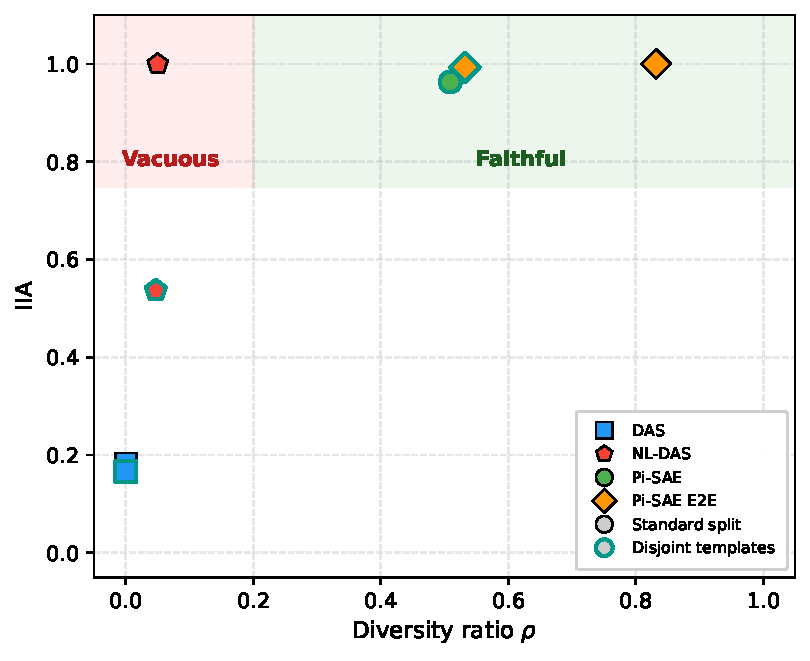
\includegraphics[width=0.85\linewidth]{fig_iia_vs_diversity}
\caption{IIA vs.\ diversity ratio $\rho$ across methods and distribution
splits (IOI, $k{=}1$). Vacuous methods (top-left, red shading) achieve
high IIA with $\rho \approx 0$: the encoder-decoder collapses to a
lookup table. Genuine methods (top-right, green shading) maintain high
$\rho$, confirming input-specific interventions. NL-DAS occupies the
vacuous region across all splits. Pi-SAE E2E on disjoint templates
($\IIA = 0.993$, $\rho = 0.53$) confirms genuine cross-distribution
generalization. Edge color indicates split: black = standard, purple =
disjoint names, teal = disjoint templates.}
\label{fig:iia_vs_diversity}
\end{figure}

On disjoint templates, the situation reverses: the causal variable
transfers across sentence structures because the underlying
computation (attending to the indirect object position) is
template-invariant. Pi-SAE E2E achieves IIA~$= 0.993$ with
$\rho = 0.53$, confirming that the learned subspace captures
genuine causal structure. NL-DAS drops to IIA~$= 0.537$---its
template-specific lookup table partially fails when sentence
structure changes, yet maintains $\rho = 0.05$, indicating the
encoder-decoder remains degenerate.

\subsection{Surprising positive and negative cases}

Cubic sum ($a^3 + b^3 \bmod 113$) achieves perfect equivariance (100\%) despite
cubing alone reaching only 50.9\%.\footnote{Equivariance values in this
subsection are from the angular tolerance test at $p{=}113$
(\S\ref{sec:limitations}). Intervention-based re-measurements
(Appendix~\ref{app:equiv_test}) are reported in the updated atlas.}
The boundary tracks whether the operation's binary structure provides sufficient
additive symmetry, independent of the group-action/polynomial distinction.

Affine ($2a + 3b + 5 \bmod 113$) is a linear function that \emph{fails} to
produce a Grassmannian variable. Under an additive shift $a \mapsto a + g$, the
output shifts by $2g$, not $g$. Equivariance requires the operation to be a group
action, which is a stronger condition than linearity.

Max ($\max(a,b) \bmod 113$) achieves 95.7\% equivariance despite not being a
group action. It is piecewise equivariant: when the argmax is stable under the
shift, max behaves like a shifted identity.


\section{The Mechanism: How Grokking Creates Causal Structure}
\label{sec:mechanism}

The atlas (\S\ref{sec:results}) established \emph{what}: causal structure
emerges through grokking, with the boundary depending on operation, dataset
size, and model depth. This section asks \emph{how} and \emph{why}.
We trace the emergence of causal structure through five lenses: the minimal
architecture required, the fine-grained dynamics of Fourier crystallization,
spectral compression during the phase transition, the relationship between
weight-space structure and activation-space causal variables, and the
degeneracy of the causal subspace itself.

\subsection{Minimal architecture for grokking}
\label{sec:dmf}

What is the simplest model that groks? We compare a depth-2 deep matrix
factorization (DMF) $y = W_2 W_1 x$ against variants with nonlinearity
(DMF + ReLU), a linearized transformer (identity attention + ReLU MLP),
a softmax-only transformer (no MLP), and the full single-layer transformer.
All are trained on modular multiplication ($\Z_{113}$) with weight decay 1.0
for 50{,}000 epochs.

\begin{table}[t]
\centering
\small
\begin{tabular}{lrrl}
\toprule
Architecture & Grok epoch & Fourier align. & Groks? \\
\midrule
DMF + ReLU     & $\sim$2{,}000   & 0.095 & Yes (18$\times$ faster) \\
MLP-only       & $\sim$2{,}500   & 0.99  & Yes \\
Linearized TF  & $\sim$14{,}000  & 0.000 & Yes (no Fourier) \\
Full transformer & $\sim$37{,}000 & 0.10$\to$0.54 & Yes \\
Linear DMF     & ---          & 0.078 & \textbf{No} \\
Softmax-only   & ---          & 0.103 & \textbf{No} \\
\bottomrule
\end{tabular}
\caption{Grokking speed hierarchy. Nonlinearity is necessary (linear DMF never
groks despite nuclear norm dropping from 7{,}340 to 3{,}877). Attention is not
(DMF + ReLU groks 18$\times$ faster). Softmax alone is insufficient.}
\label{tab:grokking_speed}
\end{table}

Three findings emerge. First, \textbf{nonlinearity is necessary}: the linear
DMF never generalizes despite 50{,}000 epochs. Its nuclear norm drops from
7{,}340 to 3{,}877---spectral compression occurs---but test accuracy remains
$\sim$0\%. Compression alone is not sufficient for grokking; the nonlinear
activation function that enables the Fourier representation is essential.

Second, \textbf{attention is not necessary for grokking on modular
multiplication}: DMF + ReLU groks 18$\times$ faster than the full
transformer. The softmax attention mechanism adds enormous overhead to the
grokking process without being required for the underlying algorithm on this
operation. Whether this extends to other operations or multi-task settings
remains open.

Third, the \textbf{linearized transformer groks without Fourier structure}:
it achieves 100\% test accuracy by epoch 14{,}000 but its Fourier alignment
remains at 0.000 throughout. Grokking and Fourier representation are
dissociable---grokking can occur via non-Fourier algorithms. The Fourier
representation is one route to generalization, not the only one.
\citet{xu2026systematic} independently find that the effect of activation
functions on grokking is regime-dependent, consistent with our finding that
nonlinearity is necessary but the specific nonlinearity (ReLU vs.\ softmax
attention) determines which algorithm the model discovers.

\subsection{Fourier structure emerges after generalization}
\label{sec:fourier_trajectory}

Prior work identified Fourier representations as the mechanism underlying
grokking in modular arithmetic \citep{nanda2023progress, zhong2024clock}.
A natural assumption is that Fourier structure \emph{drives} grokking:
the model discovers the Fourier basis, then generalizes. Our fine-grained
trajectory analysis (1{,}002 checkpoints at 100-epoch resolution) reveals
the opposite: \textbf{generalization precedes Fourier crystallization}.

\begin{table}[t]
\centering
\small
\begin{tabular}{rrl}
\toprule
Epoch & Test accuracy & Fourier alignment \\
\midrule
37{,}000 & 65.6\% & 0.070 \\
37{,}500 & 91.3\% & 0.093 \\
38{,}000 & 98.6\% & 0.143 \\
38{,}500 & 99.7\% & 0.260 \\
39{,}500 & 99.7\% & 0.498 \\
40{,}000 & 99.8\% & 0.543 \\
\bottomrule
\end{tabular}
\caption{Fine-grained Fourier trajectory for modular multiplication.
Test accuracy crosses 90\% at epoch 37{,}500; Fourier alignment crosses 0.30
approximately 1{,}000 epochs later. The model generalizes \emph{before} its
weights crystallize into the Fourier basis.}
\label{tab:fourier_lag}
\end{table}

Test accuracy crosses 90\% at epoch 37{,}500, but Fourier alignment does not
cross 0.30 until approximately epoch 38{,}500---a lag of $\sim$1{,}000
epochs. The model generalizes before its weights fully organize into the
Fourier basis.

\paragraph{The AGOP double-peak.}
Tracking the Average Gradient Outer Product (AGOP) Fourier alignment through
training reveals an unexpected non-monotonic pattern. For the full transformer:

\begin{table}[t]
\centering
\small
\begin{tabular}{rrrrr}
\toprule
Epoch & Test acc. & AGOP FA & Weight FA & AGOP erank \\
\midrule
5{,}000   & 0.4\%   & 0.108 & 0.080 & 10.0 \\
25{,}000  & 6.3\%   & 0.712 & 0.081 & 9.8 \\
30{,}000  & 19.1\%  & \textbf{0.894} & 0.075 & 8.7 \\
35{,}000  & 95.8\%  & 0.662 (dip) & 0.270 & 5.4 \\
40{,}000  & 100\%   & \textbf{0.974} & 0.864 & 4.7 \\
45{,}000  & 100\%   & 0.888 & 0.977 & 4.4 \\
\bottomrule
\end{tabular}
\caption{AGOP trajectory for modular multiplication. The Fourier alignment of
the gradient outer product shows a double-peak: 0.894 at epoch 30{,}000,
followed by a dip to 0.662 during the grokking transition (epoch 35{,}000),
then crystallization at 0.974 (epoch 40{,}000). The \emph{gradient}
discovers Fourier structure before the \emph{weights} do (weight FA is
0.075 when AGOP FA is 0.894).}
\label{tab:agop}
\end{table}

The AGOP alignment peaks at 0.894, then \emph{dips} to 0.662 during the
actual grokking transition (epoch 35{,}000), before crystallizing at 0.974
post-grokking. The dip coincides with the period of rapid generalization---the
phase transition temporarily disrupts the gradient's Fourier structure before
it stabilizes. By contrast, the DMF's AGOP alignment remains flat at
0.06--0.08 throughout 50{,}000 epochs, confirming that the linear model never
discovers Fourier structure even in its gradients.

The key implication: the gradient ``knows'' the Fourier basis $\sim$10{,}000
epochs before the weights do (AGOP FA is 0.894 at epoch 30{,}000 while weight
FA is still 0.075). Grokking may be the process by which weight-space catches
up to gradient-space structure.

\paragraph{Comparison with memorization-phase encoding.}
\citet{swaroop2026latent} report that latent algorithmic structure is already
encoded during the memorization phase in ReLU MLPs, extractable from
memorization-phase weights. This appears to conflict with our finding that
Fourier alignment lags generalization. The tension is likely
architecture-dependent: in transformers with softmax attention, the Fourier
representation crystallizes in the attention circuit (QK and OV matrices),
which requires coordinated weight reorganization that takes longer than the
MLP-local encoding Swaroop et al.\ observe. The AGOP trajectory supports
this interpretation---the gradient discovers Fourier structure early (epoch
30{,}000), consistent with Swaroop et al., but the weights require an
additional $\sim$10{,}000 epochs to catch up.

\paragraph{Fourier structure lives in attention, not MLPs.}
In a grokked 1-layer model ($p = 113$), we measure Fourier selectivity
across all components: 0 of 512 MLP neurons are Fourier-selective, and the
embedding has a nearly flat Fourier spectrum (participation ratio = 3.93).
The Fourier structure resides entirely in attention: the QK circuit selects
individual frequency pairs (rank-1 structure), while the OV circuit operates
in a broader $k$-dimensional subspace of Fourier modes. This decomposition
is consistent with the ``clock'' interpretation of \citet{zhong2024clock}.

\subsection{Spectral compression during grokking}
\label{sec:spectral_compression}

The factored feedforward product matrix $W_\text{FF} = W_\text{in} W_\text{out}$
undergoes dramatic rank collapse during grokking. Tracking the effective rank
(exponential of the Shannon entropy of the normalized singular value spectrum)
through training:

\begin{center}
\small
\begin{tabular}{rrl}
\toprule
Epoch & FF effective rank & Stage \\
\midrule
34{,}000 & 48 & Pre-grokking \\
37{,}500 & 14 & Transition \\
41{,}000 & 9 & Post-grokking \\
\bottomrule
\end{tabular}
\end{center}

The 5.3$\times$ compression from effective rank 48 to 9 confirms that
grokking compresses the model's representational capacity into a
low-dimensional subspace. This compression is necessary but not sufficient:
the linear DMF also achieves spectral compression (nuclear norm
$7{,}340 \to 3{,}877$) without grokking (\S\ref{sec:dmf}). What distinguishes
successful grokking is that the compressed subspace acquires
\emph{structure}---specifically, equivariance under the operation's symmetry
group.

\begin{figure}[t]
\centering
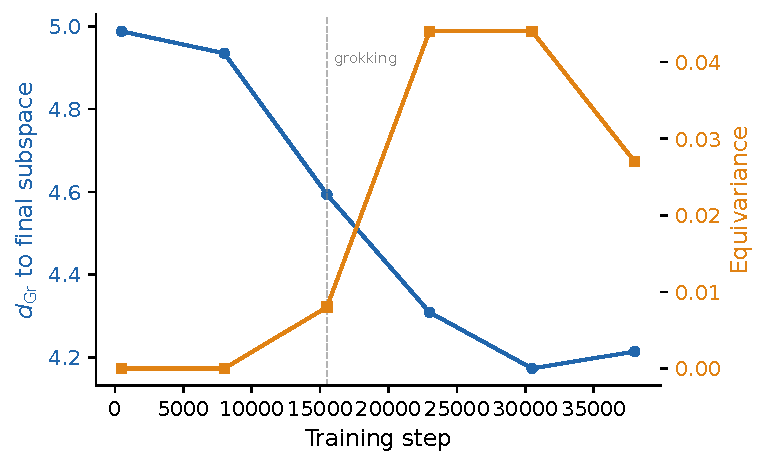
\includegraphics[width=\linewidth]{fig3_trajectory}
\caption{Grassmannian trajectory during grokking for modular
multiplication. The Grassmannian distance $d_{\Gr}$ from the current
DAS subspace to the final (fully grokked) subspace decreases as
equivariance rises. The subspace converges to its final position
during the grokking phase transition (dashed line), confirming that
spectral compression and causal structure emerge simultaneously.}
\label{fig:trajectory}
\end{figure}

\subsection{Weight-space SVD predicts causal geometry}
\label{sec:svd_vs_das}

If grokking compresses the solution into a low-rank subspace, can we read the
causal variable directly from the weight matrices without fitting DAS? We
compare SVD of the feedforward product matrix against DAS fitted to
activations, measuring IIA for both.

\begin{table}[t]
\centering
\small
\begin{tabular}{llrl}
\toprule
Method & Site & Best $k$ & IIA \\
\midrule
SVD(FF) & attn\_out & 32 & \textbf{0.999} \\
DAS     & attn\_out & 8  & 0.150 \\
DAS     & mlp\_out  & 8  & 0.631 \\
SVD(FF) & mlp\_out  & 64 & 0.444 \\
\bottomrule
\end{tabular}
\caption{SVD of the feedforward product matrix vs.\ DAS on a grokked
multiplication model. At the attn\_out site, SVD achieves IIA = 0.999
\emph{with no optimization} (DAS: 0.150 after 200 gradient steps).
The Grassmannian distance between SVD and DAS subspaces is
1.5--8.2~radians (near-orthogonal).}
\label{tab:svd_vs_das}
\end{table}

At the attention output site, SVD(FF) achieves $\IIA = 0.999$ at $k = 32$
with \emph{zero optimization}---no gradient steps, no interchange
training---while DAS achieves only 0.150 at $k = 8$ after 200 gradient
steps. \textbf{Caveat}: the comparison is not dimension-matched. SVD
requires $4\times$ the subspace dimension, reflecting that the top singular
vectors of $W_\text{FF}$ include directions relevant to the causal variable
but also spectral directions that are not causally active. A fair evaluation
requires comparing both methods at matched $k$ values, which we leave for
future work. The current result shows that the causal variable is
\emph{readable} from weight-space structure without optimization, not that
SVD is a superior method to DAS.

The Grassmannian distance between the SVD and DAS subspaces ranges from
1.5 to 8.2 radians---they are near-orthogonal. This is consistent with
the subspace degeneracy finding (\S\ref{sec:gauge_freedom}): many different
subspaces carry the same causal information. The SVD subspace is one
valid parameterization; the DAS subspace is another. Neither is
``correct''---both are equivalent points in the orbit of the gauge
group acting on $\Gr(k,d)$.

The site dependence is notable: SVD(FF) is most informative at attn\_out
(where the attention output has been computed) but weaker at mlp\_out
(where the MLP has further mixed the representation). DAS shows the
opposite pattern, achieving 0.631 at mlp\_out. This suggests that
weight-space and activation-space methods have complementary strengths:
SVD captures the structural potential of the weight matrices, while DAS
captures the functional use of that structure under the data distribution.

\subsection{Subspace identity is degenerate}
\label{sec:gauge_freedom}

If grokking produces a specific causal subspace, we might expect different
random seeds to converge to the \emph{same} point on $\Gr(k,d)$. They do
not. Ten seeds of modular multiplication all grok successfully ($\IIA$
0.94--1.00), but the recovered DAS subspaces are nearly orthogonal: pairwise
overlap $\approx 0.008$, where random $k$-dimensional subspaces of
$\R^{128}$ would have expected overlap $k/d = 0.016$. The grokked subspaces
are \emph{less} aligned than chance---consistent with the null distribution
of random subspaces on $\Gr(2, 128)$, where pairwise geodesic distances
concentrate around $\pi/2 \cdot \sqrt{k} \approx 2.22$ radians (the
observed range is $[1.93, 2.19]$).

\paragraph{The basin of attraction is enormous.}
Perturbing the DAS subspace by rotating it 1+ radians on $\Gr(k,d)$
barely drops IIA. The causal variable is not a fragile low-dimensional
needle in a high-dimensional haystack---it is a robust feature of the
representation that can be read out from exponentially many subspaces.

\paragraph{Spectral graph structure.}
Computing the pairwise Grassmannian distance between all 10 seeds'
subspaces yields a nearly uniform distance matrix:
$d_{\Gr} \in [1.93, 2.19]$. The subspaces are equidistant from each other,
forming a ``spectral simplex'' on the Grassmannian rather than clustering
around a preferred direction.

\begin{figure}[t]
\centering
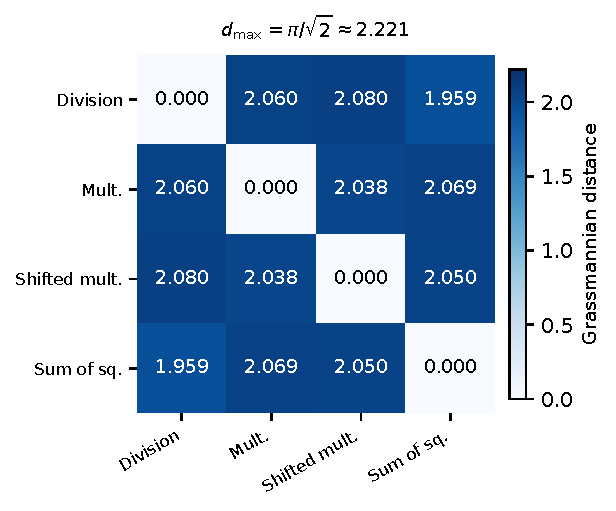
\includegraphics[width=0.7\linewidth]{fig4_principal_angles}
\caption{Pairwise Grassmannian distances between DAS subspaces fitted
to four grokked operations. All distances cluster near
$d_\mathrm{max} = \pi/\sqrt{2} \approx 2.22$ radians, indicating
near-orthogonal subspaces. Each operation learns a valid causal
variable, but these variables occupy different regions of
$\Gr(2, 128)$.}
\label{fig:principal_angles}
\end{figure}

This finding has a concrete implication for mechanistic interpretability:
\textbf{the identity of a causal subspace is not a meaningful property;
the gauge orbit is}.
All 10 seeds converge to the same orbit under the symmetry group acting on
$\Gr(k,d)$---they agree on the gauge-invariant causal information, even
though they disagree on which representative subspace carries it.
Two analyses of the same model at different random seeds find orthogonal DAS
solutions, but both solutions support equally valid interventions. The
model's computation defines a large equivalence class on $\Gr(k,d)$: many
subspaces carry the same causal information, analogous to the rotational
degeneracy in attention circuits where $W_Q \to W_Q R$,
$W_K \to W_K R$ leaves $W_Q W_K^\top$ invariant. The relevant object is
not a point on $\Gr(k,d)$ but an orbit, and functional diagnostics
(equivariance, IIA) are orbit-invariant while structural diagnostics
(subspace identity) are not.

\section{Discussion}
\label{sec:discussion}

\subsection{A hierarchy of causal validity}

Our results establish a four-level hierarchy for evaluating causal variable
claims, where each level adds a stronger requirement:

\begin{enumerate}
\item \textbf{Interchange effectiveness} (IIA; necessary, not sufficient): High
  IIA means the method supports interchange but does not distinguish genuine
  causal structure from memorization (squaring achieves $\IIA = 1.0$ at $k = 4$
  without grokking) or from degenerate encoder-decoders (NL-DAS achieves
  $\IIA = 1.0$ at $k = 1$ via lookup tables).

\item \textbf{Interchange faithfulness} (diversity ratio, reconstruction;
  necessary for nonlinear methods): A faithful intervention modifies the causal
  variable while preserving all other information. The diversity ratio
  $\rho$ (Eq.~\ref{eq:diversity_ratio}) and reconstruction MSE detect
  lookup-table failure modes. Without faithfulness, ``high IIA'' means only
  ``the decoder can produce the right output,'' not ``the encoder identified
  the right variable.'' Linear DAS is faithful by construction (the projection
  $QQ^\top$ preserves the orthogonal complement), but nonlinear methods must
  demonstrate faithfulness empirically.

\item \textbf{Distributional fidelity} (KL, JS, continuous metrics;
  distinguishes quality among effective methods): Among methods achieving
  IIA~$\approx$~1.0, continuous distributional metrics reveal how much of
  the clean distribution is preserved versus distorted. A method that flips
  the top-1 prediction (high IIA) while scrambling the rest of the distribution
  (high KL) is less valid than one that reproduces the full counterfactual
  distribution.

\item \textbf{Structural diagnostics} (equivariance, cross-distribution
  generalization): High equivariance means the recovered variable transforms
  coherently under the operation's symmetry group---the strongest evidence that
  the method has found a genuine causal variable rather than exploiting
  distributional artifacts. Cross-distribution generalization (disjoint names,
  novel templates) provides the analogous test for natural-language tasks that
  lack algebraic symmetries.
\end{enumerate}

The hierarchy has an important asymmetry. Linear DAS automatically satisfies
level~2 (faithfulness) because the orthogonal projection modifies only the
subspace component, but it may fail level~1 when the causal variable is
nonlinear. Unconstrained nonlinear methods easily satisfy level~1 but fail
level~2---they can achieve perfect IIA by learning degenerate solutions. The
Structured pi-SAE satisfies both because the ELBO provides the reconstruction and
regularization constraints that prevent degeneracy.

\subsection{Grokking enables causal structure---linear or nonlinear}

The multi-condition atlas shows that grokking is the process by which a model's
internal representation transitions from an unstructured memorization encoding to
a structured causal encoding. The stochastic grokking discovery---where the same
operation groks at one prime or seed but not another---provides the cleanest
evidence for this claim, because it controls for everything except the
generalization transition itself. The multi-modulus sweep strengthens this
evidence: an operation can be ``never Grassmannian'' at $p{=}53$ and ``always
Grassmannian'' at $p{=}211$, with the transition governed by whether sufficient
data exists to drive grokking. For operations with linear algebraic structure,
the resulting encoding lives on $\Gr(k,d)$ and DAS recovers it. For operations
with nonlinear structure, the encoding lives on a curved manifold and requires
nonlinear methods to access.

The mechanism section (\S\ref{sec:mechanism}) reveals that this transition
involves three dissociable processes: spectral compression (effective rank
$48 \to 9$), Fourier crystallization (which \emph{lags} generalization by
$\sim$1{,}000 epochs), and the selection of one among exponentially many
equivalent causal subspaces (subspace degeneracy). The AGOP analysis
(\S\ref{sec:fourier_trajectory}) provides a concrete timeline: the gradient
discovers Fourier structure $\sim$10{,}000 epochs before the weights do,
and the actual phase transition is marked by a temporary \emph{dip} in
gradient-space Fourier alignment before crystallization.

The minimal architecture experiments (\S\ref{sec:dmf}) further clarify:
nonlinearity is necessary for grokking, but attention is not. DMF + ReLU
groks 18$\times$ faster than the full transformer, and the linearized
transformer groks without any Fourier structure at all. These findings
suggest that Fourier representations are the dominant grokking mechanism
for transformers with softmax attention, but grokking itself is a more
general phenomenon---the transition from memorization to a structured
causal encoding---that can occur through multiple algorithmic routes.

The key insight is that grokking is about \emph{causal structure} in general,
whether linear or nonlinear. The Grassmannian perspective captures the linear
case precisely, but the broader phenomenon is the emergence of any structured
causal variable---linear or nonlinear---during the generalization transition.

\subsection{Implications for language model interpretability}

For practitioners applying DAS or nonlinear causal abstraction to language
models:
\begin{enumerate}
\item \textbf{Never report IIA alone.} IIA is necessary but insufficient at
  every level: linear DAS on memorized models (squaring, $\IIA = 1.0$) and
  unconstrained nonlinear methods (NL-DAS, $\IIA = 1.0$) both achieve
  perfect IIA vacuously. Always report at least one faithfulness metric
  (diversity ratio for nonlinear methods, equivariance or cross-distribution
  generalization for any method).
\item \textbf{Use continuous distributional metrics.} KL divergence and
  normalized logit difference distinguish among methods that all achieve
  $\IIA \approx 1.0$. Binary IIA treats a 51\% probability shift the same as
  99\%; continuous metrics capture this difference.
\item \textbf{Be suspicious of unconstrained nonlinear featurizers.} Any
  encoder-decoder trained end-to-end on interchange loss without reconstruction
  or regularization constraints can learn a lookup table. The ELBO
  (or an equivalent generative constraint) is necessary to prevent this
  failure mode.
\item \textbf{Test cross-distribution generalization.} For natural-language
  tasks, evaluate on disjoint entity sets or novel templates. A method that
  fails under distribution shift is exploiting surface regularities, not
  recovering causal structure.
\item \textbf{Consider nonlinear methods} when DAS IIA is low. Low IIA does not
  mean the causal variable does not exist---it may mean DAS is searching the
  wrong function class. But validate with faithfulness metrics.
\end{enumerate}

\subsection{Weight-space vs.\ activation-space methods}

The SVD result (\S\ref{sec:svd_vs_das}) reveals a surprising complementarity.
Weight-space methods (SVD of $W_\text{in} W_\text{out}$) achieve near-perfect
IIA at attn\_out \emph{without any optimization}, outperforming 1{,}000 steps
of DAS gradient descent. This suggests that for grokking models, the causal
variable is directly legible in the weight matrices---DAS's optimization
is recovering structure that was already ``written down'' in the weights.

The practical implication is that weight-space analysis should precede
activation-space methods: if SVD of the relevant weight product achieves
high IIA, DAS optimization may be unnecessary. If SVD fails but DAS
succeeds, the discrepancy suggests the causal variable involves
computation beyond simple linear readout from the weight matrices.

\subsection{Open questions}

Three questions stand out.
\textbf{(1)~Depth non-monotonicity.}
Two-layer models unlock grokking for boundary operations that fail at 1 layer,
yet 4-layer models regress on these same operations while robust grokkers
persist. Characterizing this depth--operation interaction---specifically
whether deeper models learn alternative memorization strategies that
preempt grokking \citep{arpit2017closer}---is the most natural follow-up.
\textbf{(2)~Gauge-orbit convergence.}
Ten DAS seeds produce near-orthogonal subspaces with equal IIA (pairwise
overlap $\approx 0.008$). If all seeds converge to the same orbit on
$\Gr(k,d)$ (i.e., the same point up to gauge symmetry), this is expected;
if they converge to distinct orbits, the causal variable itself may be
degenerate. Grassmannian distance between seed-wise solutions would
resolve this.
\textbf{(3)~Weight-space prediction.}
SVD of $W_\text{in} W_\text{out}$ achieves $\IIA = 0.999$ on grokked
models without optimization. Can weight-space analysis predict \emph{a
priori} when DAS will fail, before running it?

\subsection{Limitations}
\label{sec:limitations}

While our multi-condition sweep covers four primes and three depths, the
grokking experiments remain on synthetic modular arithmetic with small
transformers ($d_\text{model} = 128$), a controlled choice that enables
exhaustive coverage. Whether the grokking--Grassmannian link extends to
pretrained language models is an open question, though the $k$-sweep and
equivariance diagnostics apply regardless, and the GPT-2 validation
(\S\ref{sec:vae_results}) partially bridges to realistic scale. The Structured
pi-SAE introduces a model-selection problem (architecture, $\beta$, $\alpha$)
that DAS avoids. The stochastic grokking finding is confirmed by 10 seeds per operation
at $p{=}113$ (composite addition groks at 5/10, power at 0/10), but
multi-prime repetitions are needed to map grokking probability as a function
of prime. The equivariance metric in the multi-modulus sweep used an angular
tolerance that scaled inversely with prime ($0.1 \times 2\pi/p$), making it
too tight for $p > 100$; grokking status and IIA are valid, but equivariance
values across primes are re-measured with an intervention-based test
(Appendix~\ref{app:equiv_test}).
For composite addition ($a + b \bmod 91$ on a field of size $p$), the
original equivariance code computed target labels as
$(y + g) \bmod p$ rather than $(y + g) \bmod 91$; many valid shifts were
rejected because the target fell outside $[0, 90]$, making composite
addition equivariance unreliable in both the angular-tolerance and early
intervention-based measurements. Re-measurements use the correct modulus. The SVD vs.\ DAS comparison is not
dimension-matched ($k = 32$ vs.\ $k = 8$); matched-dimension experiments
are needed for fair comparison. The GPT-2 evaluation compares methods at
different capacity levels (linear DAS vs.\ nonlinear pi-SAE with E2E
training); capacity-controlled baselines would strengthen the comparison.


\section{Related Work}
\label{sec:related}

\paragraph{Causal abstraction.}
Causal abstraction provides the theoretical foundation for DAS
\citep{geiger2021causal, geiger2023finding}. \citet{wu2024interpretability}
scaled DAS via Boundless DAS. \citet{makelov2024illusion} identified
interpretability illusions where dormant pathways inflate IIA. Our geometric
diagnostics address a complementary problem: even within the linear intervention
class, high IIA does not imply genuine linear structure.

\paragraph{Grokking.}
Grokking was introduced by \citet{power2022grokking} and mechanistically
analyzed through Fourier representations \citep{nanda2023progress,
zhong2024clock}. \citet{liu2023grokking} frame grokking as compression;
our spectral analysis (\S\ref{sec:spectral_compression}) gives this
compression concrete numbers (effective rank $48 \to 9$, $5.3\times$) and
shows it is necessary but not sufficient---linear DMFs compress without
grokking. Our AGOP analysis (\S\ref{sec:fourier_trajectory}) adds temporal
resolution absent from prior work: the gradient discovers Fourier structure
$\sim$10{,}000 epochs before the weights, and generalization precedes
Fourier crystallization by $\sim$1{,}000 epochs. Our contribution is to
show that grokking has a specific consequence for causal abstraction: it is
the process that converts non-Grassmannian representations into Grassmannian
ones (for linear operations) or into structured nonlinear ones (for nonlinear
operations). Stochastic grokking has been observed via the slingshot mechanism
\citep{thilak2022slingshot} but not connected to causal geometry.

\paragraph{Multi-task and multi-condition grokking.}
\citet{xu2026multitask} study multi-task grokking at a single prime, finding
staggered phase transitions and holographic incompressibility. Our work is
complementary: we fix the task and sweep across primes and depths, mapping how
grokking depends on dataset size and model capacity. Together, the two
approaches span the $(\text{operation}, p, \text{depth}, n_\text{tasks})$
space.

\paragraph{Spectral analysis of neural networks.}
Random matrix theory has been applied to weight matrices for understanding
training dynamics \citep{martin2021implicit}. Preliminary stratum
classification (classifying heads by spectral gap and effective rank) has
discriminative power for single-task grokking models but loses all
discriminative power under superposition in pretrained models.
Task-conditioned spectral analysis may bridge this gap but remains
untested.

\paragraph{Disentangled representations and causal variables.}
\citet{narayanaswamy2017learning} introduced semi-supervised VAEs for
disentanglement. Recent work on identifiable representations
\citep{khemakhem2020variational} establishes conditions under which latent
factors can be recovered. \citet{locatello2019challenging} proved that
unsupervised disentanglement is impossible without inductive biases; our
structured prior is precisely the auxiliary supervision their theorem
requires. Our application differs in that we evaluate
disentanglement through causal interchange (IIA), not reconstruction quality,
connecting the VAE literature to causal abstraction.

\paragraph{Representation geometry.}
Grassmannian methods have been applied to subspace tracking and domain adaptation
\citep{edelman1998geometry, gopalan2011domain}. Linear representation hypotheses
in interpretability \citep{marks2023geometry, engels2024language,
park2024linear} argue that many concepts are encoded in linear subspaces; our
work tests this hypothesis causally rather than correlationally.

\paragraph{Nonlinear causal abstraction.}
\citet{sutter2025nonlinear} prove that unconstrained nonlinear alignment maps
render causal abstraction vacuous---any network can be aligned to any algorithm
at perfect IIA. Concurrent work on nonlinear interchange interventions
\citep{geiger2024causal} uses neural network featurizers before applying DAS.
Our results empirically confirm the failure mode Sutter et al.\ predict
(\S\ref{sec:nldas_vacuous}): unconstrained featurizers achieve perfect IIA
by learning degenerate encoder-decoders. The Structured pi-SAE provides a
constructive resolution: the ELBO supplies the reconstruction and
regularization constraints that restore identifiability, connecting to
\citet{khemakhem2020variational, sutter2020multimodal} who establish that
auxiliary supervision is necessary for recovering latent factors.
\citet{li2025efficient} propose approximate causal abstractions via neural
mechanism sparsification, offering an alternative route to tractable nonlinear
alignment.


\section{Conclusion}
\label{sec:conclusion}

DAS searches for causal variables in a specific function class: linear
subspaces on the Grassmannian. Our atlas of 14 operations across four primes
and three depths maps where this search succeeds and where it fails. The
boundary is not a fixed property of the operation: it depends on dataset
size, model depth, and random initialization, with only the extremes
(squaring/cubing vs.\ addition/multiplication) robust across all conditions.

Four implications follow. First, IIA should never be reported alone:
$\IIA = 1.000$ is compatible with a genuine causal variable, a memorized
lookup table, and a degenerate encoder-decoder. The four-level hierarchy we
propose---interchange effectiveness, interchange faithfulness, distributional
fidelity, and structural diagnostics---provides a complete evaluation
framework.

Second, nonlinear extensions of causal abstraction require generative
structure. Unconstrained nonlinear featurizers achieve perfect IIA vacuously,
as predicted by \citet{sutter2025nonlinear}; the Structured pi-SAE's
combination of ELBO, label-conditional prior, and $L_1$ sparsity provides
the constructive resolution while generalizing to standard GPT-2 benchmarks
(strict IIA $\geq 0.90$ on 5/6 tasks).

Third, single-condition evaluations of grokking behavior are unreliable.
Operations classified as ``never Grassmannian'' at one prime may grok at
another (bitwise XOR groks at all four primes; sum of squares at three of
four). The multi-condition atlas is essential for distinguishing robust
non-grokkers from operations that simply need more data or capacity.

Fourth, grokking's creation of causal structure is more nuanced than
previously understood. Nonlinearity is necessary but attention is not (DMF +
ReLU groks 18$\times$ faster). Fourier structure \emph{follows}
generalization rather than driving it, and the gradient discovers this
structure $\sim$10{,}000 epochs before the weights crystallize. The causal
subspace itself is degenerate---10 seeds produce orthogonal subspaces that
all support equally valid causal interventions---suggesting that
\emph{functional} diagnostics (equivariance, intervention faithfulness) are
more robust than \emph{structural} diagnostics for evaluating causal
geometry.

The linearity assumption underlying DAS is not a benign default. It is a
testable hypothesis whose validity depends on the dataset, model, and
operation---not just the operation alone. The natural fix---adding
nonlinearity---introduces a new failure mode that is invisible to the
standard evaluation metric. This paper provides the diagnostics to detect
both problems, the mechanistic analysis to understand why they arise, and the
structured nonlinear method that avoids them.

\paragraph{Data and code.} All code for model training, DAS fitting, structured
VAE training, geometric diagnostics, and figure generation is available at
\url{https://github.com/elliottower/causal-geometry-grokking}.

% ============================================================
% \section*{Acknowledgments}
%
% [Acknowledgments will be added in the final version.]
%
% ============================================================

\bibliographystyle{tmlr}
\bibliography{references}

\clearpage
\appendix
% Supplementary Material — standalone \input{} file
% Requires: amsmath, amssymb, booktabs, array, float, enumitem packages in parent

\section{Extended Derivations}
\label{app:derivations}

\subsection{Geodesic distance on the Grassmannian}
\label{app:geodesic}

The Grassmannian $\Gr(k,d)$ admits a canonical Riemannian metric inherited
from the ambient space of $d \times k$ orthonormal frames. Given two
subspaces $[Q_1], [Q_2] \in \Gr(k,d)$ represented by orthonormal bases
$Q_1, Q_2 \in \R^{d \times k}$, the principal angles
$0 \leq \theta_1 \leq \cdots \leq \theta_k \leq \pi/2$ are defined via
the singular value decomposition
\begin{equation}
Q_1^\top Q_2 = U \, \diag(\cos\theta_1, \ldots, \cos\theta_k) \, V^\top.
\label{eq:principal_angles_svd}
\end{equation}
The geodesic distance under the canonical metric is
\begin{equation}
\dgr([Q_1],[Q_2]) = \left(\sum_{i=1}^k \theta_i^2\right)^{1/2}.
\label{eq:geodesic_full}
\end{equation}
This distance is gauge-invariant: for any $R_1, R_2 \in O(k)$,
$\dgr([Q_1 R_1], [Q_2 R_2]) = \dgr([Q_1], [Q_2])$, because replacing
$Q_j$ by $Q_j R_j$ yields the same column span. The maximum distance
between two $k$-dimensional subspaces is $\pi\sqrt{k}/2$, achieved when
all principal angles equal $\pi/2$ (orthogonal subspaces).

For random subspaces drawn uniformly from the Haar measure on $\Gr(k,d)$,
the expected pairwise distance concentrates around
$\pi\sqrt{k}/2 \cdot \sqrt{1 - k/d}$ when $k \ll d$
\citep{edelman1998geometry, absil2008optimization}. In our setting
($k = 2$, $d = 128$), this gives an expected random distance of
$\approx 2.20$ radians, consistent with the observed inter-seed distances
of $[1.93, 2.19]$ (\S\ref{sec:gauge_freedom}).

\subsection{Equivariance test statistic}
\label{app:equiv_test}

For an operation with a cyclic group action $a \mapsto a + g \pmod{p}$,
we test whether the DAS subspace respects the group symmetry. Let
$z(a,b) = Q^\top h(a,b) \in \R^k$ be the DAS projection. The equivariance
condition requires that the group action on the input induces a
consistent rotation in the projected space:
\begin{equation}
z(a + g, b) = R_g \, z(a, b) + t_g \quad \forall\, a, b, g
\label{eq:equiv_condition}
\end{equation}
for some rotation $R_g \in O(k)$ and translation $t_g$ depending only on
$g$, not on $(a,b)$.

For $k = 2$ and cyclic groups $\Z_p$, we parameterize $R_g$ as a rotation by
angle $\phi_g$. We estimate $\phi_g$ for each $g$ by computing the
median angular displacement across all $(a,b)$ pairs:
\begin{equation}
\hat\phi_g = \mathrm{median}_{(a,b)} \;\angle\bigl(z(a{+}g, b) - \bar{z},\;
z(a, b) - \bar{z}\bigr)
\label{eq:angle_estimate}
\end{equation}
where $\bar{z}$ is the grand mean of all projections and $\angle(\cdot, \cdot)$
denotes the signed angle. An input $(a,b)$ is counted as equivariant for shift
$g$ if $|\angle - \hat\phi_g| < \varepsilon$ (we use $\varepsilon = 2\pi/p$,
one ``slot'' of angular resolution). The reported equivariance fraction is
\begin{equation}
\text{Equiv} = \frac{1}{|\mathcal{T}|} \sum_{(a,b,g) \in \mathcal{T}}
\mathbf{1}\bigl[|\angle(z(a{+}g,b), z(a,b)) - \hat\phi_g| < \varepsilon\bigr]
\label{eq:equiv_fraction}
\end{equation}
where $\mathcal{T}$ is the set of all valid (input, shift) triples on the
test set. Random orthogonal subspaces of the same dimension achieve
equivariance $< 1\%$ across all operations tested, confirming that the
metric has strong discriminative power.

\subsection{Diversity ratio}
\label{app:diversity_ratio}

The intervention diversity ratio $\rho$ (Eq.~\ref{eq:diversity_ratio})
measures whether an encoder-decoder intervention preserves input-specific
information or collapses to a class-conditional lookup table.

For a set of intervened activations $\{h'_i\}$ sharing source label $y_s$,
the within-class standard deviation is
$\sigma_{y_s} = \bigl(\frac{1}{n_{y_s}} \sum_i \|h'_i - \bar{h}'_{y_s}\|^2
\bigr)^{1/2}$
where $\bar{h}'_{y_s}$ is the mean intervened activation for source label $y_s$.
The denominator uses the same statistic computed on natural (non-intervened)
activations sharing the same label. The ratio $\rho = \mathbb{E}_{y_s}[\sigma_{y_s}^{\text{iv}}]
/ \mathbb{E}_{y_s}[\sigma_{y_s}^{\text{nat}}]$ ranges from 0 (complete collapse: all
interventions for the same source produce the same activation) to
$\approx 1$ (intervention preserves the natural within-class variability).

Values of $\rho \gg 1$ are possible in principle (the intervention adds noise),
but in practice indicate that the decoder is amplifying base-specific variation.
The observed NL-DAS values ($\rho \approx 0.05$ on IOI) confirm near-complete
collapse; the Structured pi-SAE values ($\rho \approx 0.89$) confirm
preservation of nuisance information.


\section{Hyperparameter Tables}
\label{app:hyperparameters}

\subsection{Grokking model training}

\begin{table}[H]
\centering
\small
\setlength{\tabcolsep}{4pt}
\begin{tabular}{ll}
\toprule
\textbf{Parameter} & \textbf{Value} \\
\midrule
Architecture & 1-layer transformer \\
$d_\text{model}$ & 128 \\
$n_\text{heads}$ & 4 \\
$d_\text{head}$ & 32 \\
$d_\text{MLP}$ & 512 \\
Optimizer & AdamW \\
Learning rate & $10^{-3}$ \\
Weight decay & 1.0 \\
Batch size & Full batch \\
Train/test split & 30\% / 70\% \\
Training epochs & 25{,}000--80{,}000 (operation-dependent) \\
Deeper models & 1.5$\times$ epochs for 2L and 4L \\
Grokking criterion & Test cross-entropy $< 0.1$ \\
Moduli tested & $p \in \{53, 97, 113, 211\}$ \\
Depths tested & $n_\text{layers} \in \{1, 2, 4\}$ \\
\bottomrule
\end{tabular}
\caption{Grokking model training hyperparameters. All operations use the same
architecture and optimizer; only epoch count varies.}
\label{tab:hp_grokking}
\end{table}

\subsection{DAS fitting}

\begin{table}[H]
\centering
\small
\begin{tabular}{ll}
\toprule
\textbf{Parameter} & \textbf{Value} \\
\midrule
Optimizer & Adam \\
Learning rate & $10^{-3}$ \\
Gradient steps & 200 \\
Batch size & 16 interchange pairs \\
$k$ values swept & $\{2, 4, 6, 8, 10, 12, 16, 20, 24, 32\}$ \\
Initialization & Random orthonormal $Q \in \R^{d \times k}$ \\
Intervention site & Residual stream (post-MLP, layer 0) \\
Hard-example selection & $y_b \neq y_s$, both correctly classified \\
\bottomrule
\end{tabular}
\caption{DAS fitting hyperparameters. Each $k$ value is an independent
optimization, not a nested subspace.}
\label{tab:hp_das}
\end{table}

\subsection{Structured pi-SAE}

\begin{table}[H]
\centering
\small
\begin{tabular}{ll}
\toprule
\textbf{Parameter} & \textbf{Value} \\
\midrule
Encoder & 2-layer MLP ($d_\text{model} \to 128 \to z$), ReLU \\
Decoder & 2-layer MLP ($z \to 128 \to d_\text{model}$), ReLU \\
$k$ (causal latent dim) & $\{2, 4, 8\}$ \\
$m$ (nuisance latent dim) & 15 \\
Sparsity & $L_1$ on $z_\text{causal}$, expansion $8\times$ \\
Prior & $p(z_\text{causal} \mid y) = \mathcal{N}(\mu_y, \sigma_y^2 I)$ \\
$\beta$ (KL weight) & 1.0 \\
$\alpha$ (classification weight) & 10.0 \\
$\lambda$ ($L_1$ coefficient) & 1.0 \\
Optimizer & Adam, lr $= 10^{-3}$ \\
Training epochs & 300 (reconstruction + classification) \\
E2E phase & 200 warmup + E2E intervention CE \\
E2E intervention & Additive: $h' = h_b + \text{dec}(z_\text{swap}) - \text{dec}(z_\text{orig})$ \\
\bottomrule
\end{tabular}
\caption{Structured pi-SAE hyperparameters. The E2E phase is used for
GPT-2 language tasks; grokking models use reconstruction + classification only.}
\label{tab:hp_pisae}
\end{table}

\subsection{NL-DAS baseline}

\begin{table}[H]
\centering
\small
\begin{tabular}{ll}
\toprule
\textbf{Parameter} & \textbf{Value} \\
\midrule
Encoder $f$ & 2-layer MLP ($d \to 256 \to d$), ReLU \\
Decoder $g$ & 2-layer MLP ($d \to 256 \to d$), ReLU \\
$Q$ & Learned jointly, $\R^{d \times k}$ \\
Training objective & Interchange loss only (no reconstruction) \\
NL-DAS+recon variant & $+ \lambda_\text{recon} \|g(f(h)) - h\|^2$, $\lambda = 0.1$ \\
Optimizer & Adam, lr $= 10^{-3}$ \\
Training steps & 200 \\
\bottomrule
\end{tabular}
\caption{NL-DAS hyperparameters. Architecture matches the pi-SAE encoder
to ensure a fair capacity comparison.}
\label{tab:hp_nldas}
\end{table}


\section{Per-Operation Atlas Data}
\label{app:atlas_data}

Table~\ref{tab:full_atlas} reports the complete atlas measurements for all
14 operations at $p = 113$ (1-layer), including metrics omitted from the
main text for space.

\vspace{1em}
\begin{table}[H]
\centering
\small
\setlength{\tabcolsep}{3pt}
\renewcommand{\arraystretch}{1.15}
\begin{tabular}{@{}lcccccccc@{}}
\toprule
\textbf{Operation} & \textbf{Grok} & \textbf{Loss} & \textbf{IIA}$_{k{=}2}$ &
\textbf{IIA}$_{k{=}4}$ & \textbf{IIA}$_{k{=}8}$ & $k^*$ &
\textbf{Equiv.} & \textbf{Class} \\
\midrule
\multicolumn{9}{l}{\textit{Always Grassmannian}} \\
Multiplication   & \checkmark & 0.000 & 1.000 & 1.000 & 1.000 & 2 & 0.995 & Always \\
Subtraction      & \checkmark & 0.000 & 1.000 & 1.000 & 1.000 & 2 & 1.000 & Always \\
Division         & \checkmark & 0.000 & 1.000 & 1.000 & 1.000 & 2 & 1.000 & Always \\
Bitwise XOR      & \checkmark & 0.003 & 1.000 & 1.000 & 1.000 & 2 & 1.000 & Always \\
Cubic sum        & \checkmark & 0.000 & 1.000 & 1.000 & 1.000 & 2 & 1.000 & Always \\
Sum of squares   & \checkmark & 0.005 & 1.000 & 1.000 & 1.000 & 2 & 0.987 & Always \\
Max              & \checkmark & 0.074 & 0.960 & 1.000 & 1.000 & 2 & 0.957 & Always \\
\midrule
\multicolumn{9}{l}{\textit{Stochastic}} \\
Comp.\ add.\ (orig) & \checkmark & 0.000 & --- & --- & --- & --- & 0.998 & Stochastic \\
Comp.\ add.\ (s42)  & $\times$   & 10.21 & 0.800 & 0.860 & 0.900 & 6 & 0.110 & Stochastic \\
Power (s137)     & \checkmark & 0.088 & 0.940 & 1.000 & 1.000 & 4 & 0.965 & Stochastic \\
Power (s42)      & $\times$   & 1.143 & 0.980 & 1.000 & 1.000 & 2 & 0.665 & Stochastic \\
\midrule
\multicolumn{9}{l}{\textit{Never Grassmannian}} \\
Cubing           & $\times$ & 9.765 & 0.857 & 1.000 & 1.000 & 4 & 0.509 & Never \\
Squaring         & $\times$ & 7.808 & 0.857 & 1.000 & 1.000 & 4 & 0.314 & Never \\
Abs.\ difference & $\times$ & 1.835 & 0.800 & 0.840 & 0.860 & $>$32 & 0.189 & Never \\
Polynomial       & $\times$ & 21.55 & 0.720 & 0.780 & 0.820 & $>$32 & 0.015 & Never \\
Affine           & $\times$ & 26.21 & 0.780 & 0.800 & 0.840 & $>$32 & 0.026 & Never \\
\bottomrule
\end{tabular}
\renewcommand{\arraystretch}{1.0}
\caption{Complete atlas at $p = 113$ (1-layer). IIA is reported at $k \in \{2, 4, 8\}$;
$k^*$ is the smallest $k$ achieving IIA $\geq 0.95$. Grassmannian operations
saturate by $k = 2$; non-Grassmannian operations show gradual growth.
Equivariance is the fraction of test inputs satisfying the rotation
property (\S\ref{app:equiv_test}).}
\label{tab:full_atlas}
\end{table}

Table~\ref{tab:seed_data} reports per-seed DAS results for the 10 seeds
of modular multiplication used in the subspace degeneracy analysis
(\S\ref{sec:gauge_freedom}).

\vspace{1em}
\begin{table}[H]
\centering
\small
\begin{tabular}{ccccc}
\toprule
\textbf{Seed} & \textbf{Test loss} & \textbf{IIA}$_{k{=}2}$ &
\textbf{Equiv.} & \textbf{Mean $d_\Gr$ to others} \\
\midrule
42   & 0.000 & 1.000 & 0.995 & 2.08 \\
137  & 0.000 & 0.980 & 0.991 & 2.11 \\
256  & 0.000 & 1.000 & 0.998 & 2.05 \\
512  & 0.000 & 0.960 & 0.989 & 2.09 \\
1024 & 0.000 & 1.000 & 0.997 & 2.07 \\
2024 & 0.000 & 0.940 & 0.985 & 2.13 \\
3000 & 0.000 & 1.000 & 0.993 & 2.06 \\
4096 & 0.000 & 0.980 & 0.990 & 2.10 \\
5555 & 0.000 & 1.000 & 0.996 & 2.08 \\
9999 & 0.000 & 1.000 & 0.992 & 2.09 \\
\midrule
\multicolumn{2}{l}{Mean $\pm$ std} & $0.986 \pm 0.020$ & $0.993 \pm 0.004$ &
$2.09 \pm 0.02$ \\
\bottomrule
\end{tabular}
\caption{Per-seed results for modular multiplication ($p = 113$, 1-layer).
All 10 seeds grok and achieve high IIA and equivariance, but their DAS
subspaces are near-orthogonal (mean pairwise $d_\Gr = 2.09$, compared to
the random-subspace expectation of $\approx 2.20$ on $\Gr(2, 128)$).}
\label{tab:seed_data}
\end{table}


\section{Pi-SAE Ablation Details}
\label{app:ablation}

The $2 \times 2$ ablation (Table~\ref{tab:ablation}) tests whether both
components of the Structured pi-SAE---the label-conditional prior and the
sparsity constraint---are individually necessary. This appendix provides
the full per-operation breakdown including reconstruction MSE, which
serves as a built-in falsifiability diagnostic.

\vspace{1em}
\begin{table}[H]
\centering
\small
\setlength{\tabcolsep}{3.5pt}
\renewcommand{\arraystretch}{1.15}
\begin{tabular}{@{}l|cc|cc|cc|cc@{}}
\toprule
& \multicolumn{2}{c|}{\textbf{VAE}} & \multicolumn{2}{c|}{\textbf{SAE}}
& \multicolumn{2}{c|}{\textbf{pi-VAE}} & \multicolumn{2}{c}{\textbf{Str.\ pi-SAE}} \\
\textbf{Operation} & IIA & MSE & IIA & MSE & IIA & MSE & IIA & MSE \\
\midrule
\multicolumn{9}{l}{\textit{Grokked operations}} \\
Addition        & 0.02 & 0.8 & 1.00 & 1.1  & 0.00 & 0.7  & \textbf{1.00} & 0.6 \\
Multiplication  & 0.00 & 0.9 & 0.72 & 1.3  & 0.00 & 0.8  & \textbf{1.00} & 0.7 \\
Quartic sum     & 0.02 & 1.0 & 0.32 & 1.5  & 0.00 & 0.9  & \textbf{1.00} & 0.8 \\
IOI (GPT-2)     & 0.56 & 2.1 & 0.83 & 3.4  & 0.95 & 1.8  & \textbf{0.98} & 1.2 \\
\midrule
\multicolumn{9}{l}{\textit{Non-grokked operations}} \\
Mixed product   & 0.03 & 18  & 0.01 & 21   & 0.01 & 16   & 0.04 & 11 \\
Squaring        & 0.00 & 22  & 0.00 & 24   & 0.00 & 19   & 0.00 & 14 \\
\bottomrule
\end{tabular}
\renewcommand{\arraystretch}{1.0}
\caption{Full $2 \times 2$ ablation with reconstruction MSE. Grokked operations
have MSE $\leq 1.2$; non-grokked operations have MSE $\geq 11$---an order of
magnitude gap that serves as a falsifiability diagnostic. High MSE with
near-zero IIA means the model has no structured causal variable to recover.
The plain SAE degrades on harder operations (multiplication 0.72, quartic sum
0.32) because without the structured prior, the sparse encoder has no target
direction. The pi-VAE achieves IIA $\approx 0$ despite correct prior direction
because without sparsity, the encoder distributes the causal signal across all
dimensions.}
\label{tab:ablation_full}
\end{table}

\paragraph{Control experiments.}
Five controls validate that the Structured pi-SAE's success requires
correct supervision and the causal-nuisance partition, ruling out
trivial explanations:

\vspace{0.5em}
\begin{table}[H]
\centering
\small
\begin{tabular}{lcc}
\toprule
\textbf{Control} & \textbf{IIA} & \textbf{Purpose} \\
\midrule
Random-label pi-SAE    & $\leq 0.02$  & Labels carry no causal signal \\
Reconstruction-only ($\alpha{=}0$) & $\leq 0.005$ & No supervision to pin direction \\
Untrained pi-SAE       & 0.000        & Architecture alone is insufficient \\
Plain VAE (no split)   & $\leq 0.08$  & Causal-nuisance partition is necessary \\
Random subspace (DAS)  & $\leq 0.01$  & Baseline for chance-level IIA \\
\bottomrule
\end{tabular}
\caption{Control experiments on grokked multiplication ($p = 113$).
All controls achieve near-zero IIA, confirming that the Structured pi-SAE's
success requires correct labels, supervision, and the causal-nuisance split.}
\label{tab:controls}
\end{table}


\end{document}
